\chapter{ Results \& Discussion}

A brief summary of the key observation and associated implications are presented here. First the effect of forcing Strouhal number is summarized. Following this the changes to the flow field while forcing at a single Strouhal number is presented in detail, to highlight exmplemary features of the forced flow.

\section{Effect of Strouhal Number}

A range of Strouhal numbers $St= f_fb/V_j = b/\lambda_j \approx 0.28 - 5.7 \times 10^{-3}$ were considered. Here, $\lambda_j$ is the forcing wavelength based on the PWJ jet exit height $b$. The focus is specifically on changes to the wall shear stress $\tau_w$ or skin friction. The reduction in wall shear stress, is shown here as a reduction in friction velocity $U_\tau=\sqrt{\tau_w/\rho}$. This is shown as a function of forcing Strouhal number as well as streamwise location in Figure~\ref{fg:uTauStNum}. A reduction in the wall-shear stress was observed for all excitation wavelengths, as well as for all streamwise distances considered. It is seen that for all the streamwise distances considered there is a specific wavelength ($\approx 3.3 \times 10^{-3} b/\lambda_j$, $\lambda_j = V_j/b f_{f}$) at which a clear maximum reduction in friction velocity $U_\tau$ is obtained. This wavelength is independent of downstream distance though the actual \% reduction in $U_\tau$ is a function of downstream distance. The maximum reduction in $U_\tau$ was at a downstream distance of $x/b=100$ after which the reduction decreases for all downstream distances considered. 

\begin{figure}[H]
	\centering
	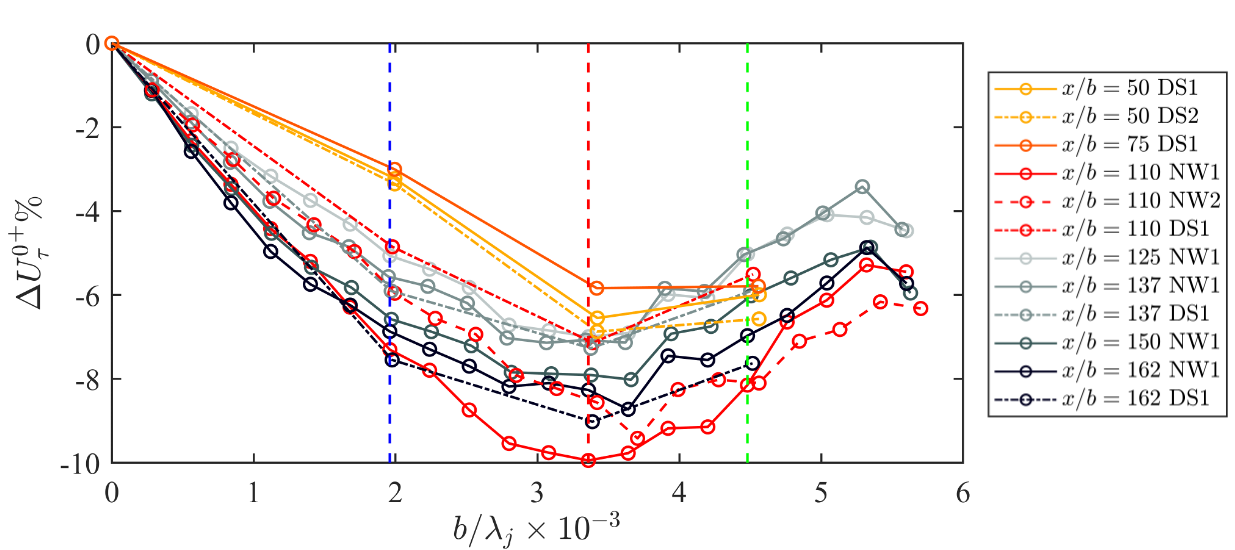
\includegraphics[width=.99\textwidth]{pics/uTauStNum.png}
	\caption{The reduction in friction velocity $\Delta U_{\tau}$ as a function of the Strouhal number $St = b/\lambda_j$ at various streamwise locations. The vertical dashed lines show the forcing frequencies $f_{f} = 7$ Hz (\textcolor{blue}{\dashed}), $f_{f} = 12$ Hz (\textcolor{red}{\dashed}) and $f_{f} = 16$ Hz (\textcolor{green}{\dashed}) respectively. Detailed results from $f_f=7$ Hz is presented in this report.}
	\label{fg:uTauStNum}
\end{figure}


Results presented in this report are primarily from forcing at $f_f=7$ Hz (blue line in Figure~\ref{fg:uTauStNum}). This case is referred to here on as case A. The internal mechanisms of the PWJ at this forcing was representative of the behavior at other forcing frequencies. At this forcing frequency $f_f=7$ Hz, the perturbation wavelength was $\lambda_{xf}\approx 6.6 \delta$ (based on the outer scales at the downstream location $x/b=137$). In this case, the perturbation increased the turbulence intensity at the PWJ exit centerline from $<1\%$ to $5.5\%$, making it a large-amplitude forcing. Other forcing frequencies $f_f=$ 12 (referred to as case B) and 16 Hz (referred to as case C) where also studied in detail and are briefly presented here and in greater detail in the publications and dissertations funded by this work. 

\section{Mean Flow Statistics}

\begin{figure}[H]
	\centering
	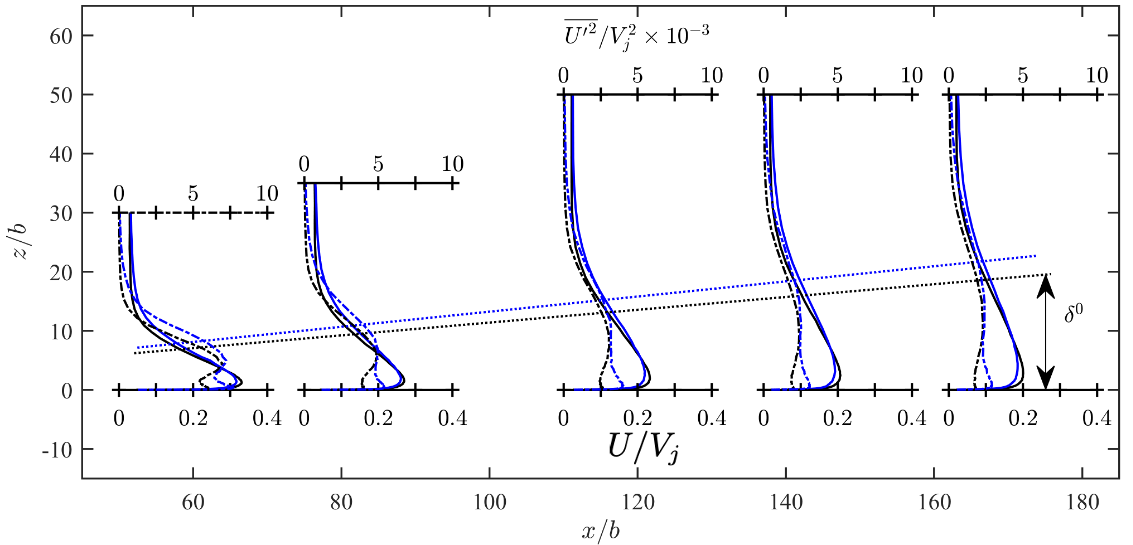
\includegraphics[width=.95\textwidth]{pics/meanVelTurbInt.png}
	\caption{The solid lines show the mean effective streamwise velocity profile ${U}$ as measured by HWA as the flow develops downstream of the PWJ exit. The dot-dashed line shows the corresponding evolution of the effective streamwise turbulence intensity $\overline{U^{\prime2}}$ profiles. The black lines are those corresponding to the unperturbed PWJ while the blue ones are those corresponding to the perturbed PWJ (case A). The development of the outer length scale $\delta$ is also shown indicating the spreading rate of the PWJ.}
	\label{fg:meanVelTurbInt}
\end{figure}

\begin{figure}[h]
	\centering
	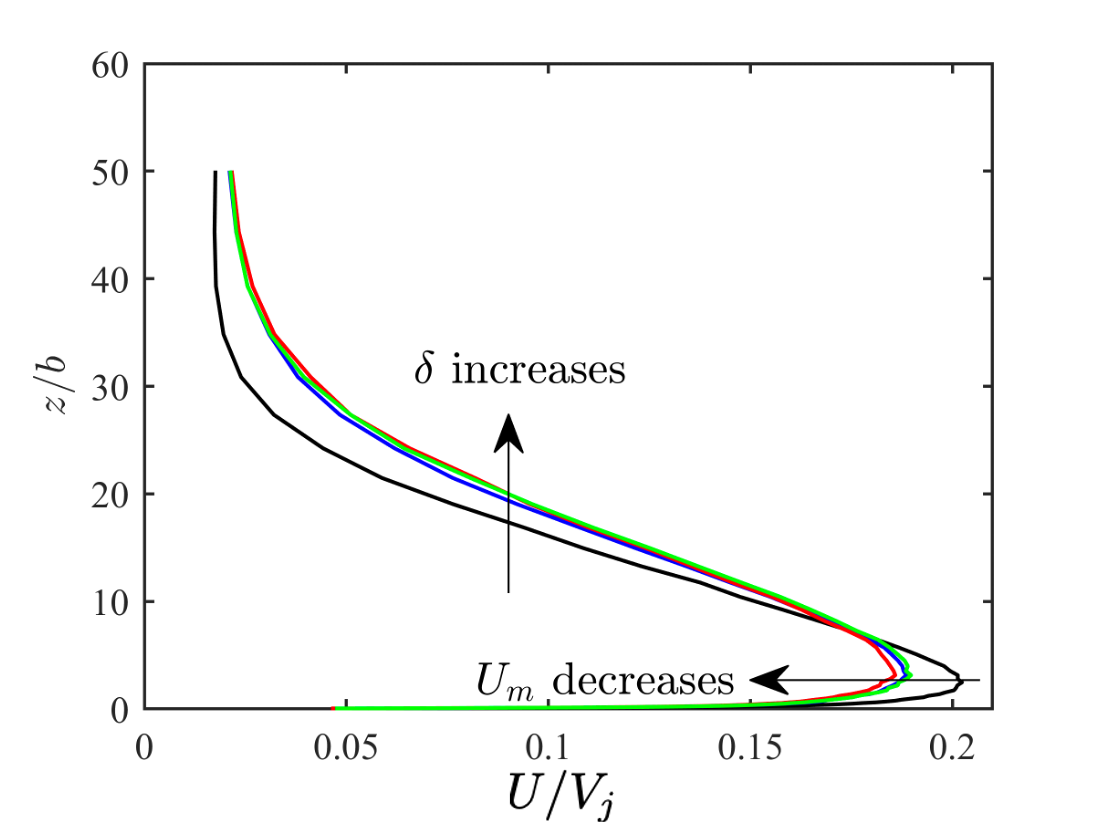
\includegraphics[width=.65\textwidth]{pics/meanVel137.png}
	\caption{Mean velocity profiles at $x/b = 137$ for the unforced flow (\textcolor{black}{\full}) and the forced flow; case A (\textcolor{blue}{\full}), case B (\textcolor{red}{\full}) and case C (\textcolor{green}{\full}).}
	\label{fg:meanVel137}
\end{figure}

\begin{figure}[h!]
	\centering
	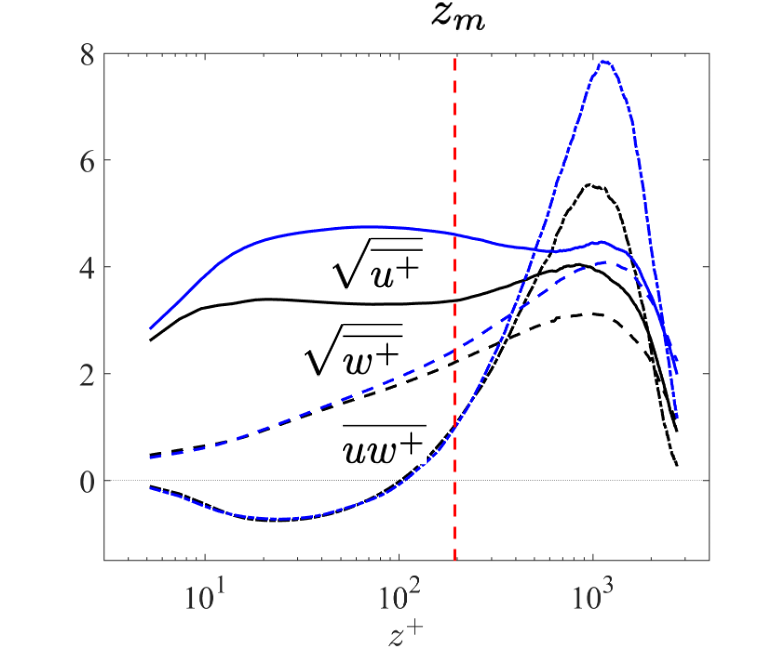
\includegraphics[width=.65\textwidth]{pics/turbInt137.png}
	\caption{Turbulent stresses at $x/b=137$ from PIV measurements for the unforced (black lines) and the case A forced flow (blue lines).}
	\label{fg:turbInt137}
\end{figure}

The streamwise evolution of the mean velocity as well as the turbulence intensity as measured by HWA is shown in Figure~\ref{fg:meanVelTurbInt}. The mean velocity at $x/b=137$ comparing the three different forcing highlighted in Figure~\ref{fg:uTauStNum} is also shown. The maximum velocity, the outer velocity scale, $U_m$ is reduced when the PWJ is forced. The outer length scale $\delta$ or the shear layer thickness on the other hand increases upon forcing. These large-scale changes together along with the decrease in $U_\tau$ increases the local Reynolds number $Re_\tau=u_\tau \delta/\nu$ when forced. 

The turbulence intensity of the unforced PWJ has two peaks one in the inner wall region and the other in outer jet region. This is seen in Figure~\ref{fg:turbInt137} which shows the PIV based turbulence intensity at $x/b=137$. The streamwise turbulence intensity in the inner wall region is increased considerably by the forcing. There is a smaller increase in the outer jet region. On the other hand there is little change in the spanwise turbulence intensity in the wall region, with a gradual increase moving outwards reaching a maximum increase in the jet region, coinciding with the location of the outer peak of the unforced flow. Similarly, the Reynolds shear stress shows virtually no change in the inner wall region but has an increase with a maximum increase around the outer peak. The streamwise evolution of the turbulence intensity as measured by HWA is shown also in Figure~\ref{fg:meanVelTurbInt}. The behavior at $x/b=137$, is shown to be typical of all other streamwise locations considered.

\section{Skin friction and Momentum}

\begin{figure}[h!]
	\centering
	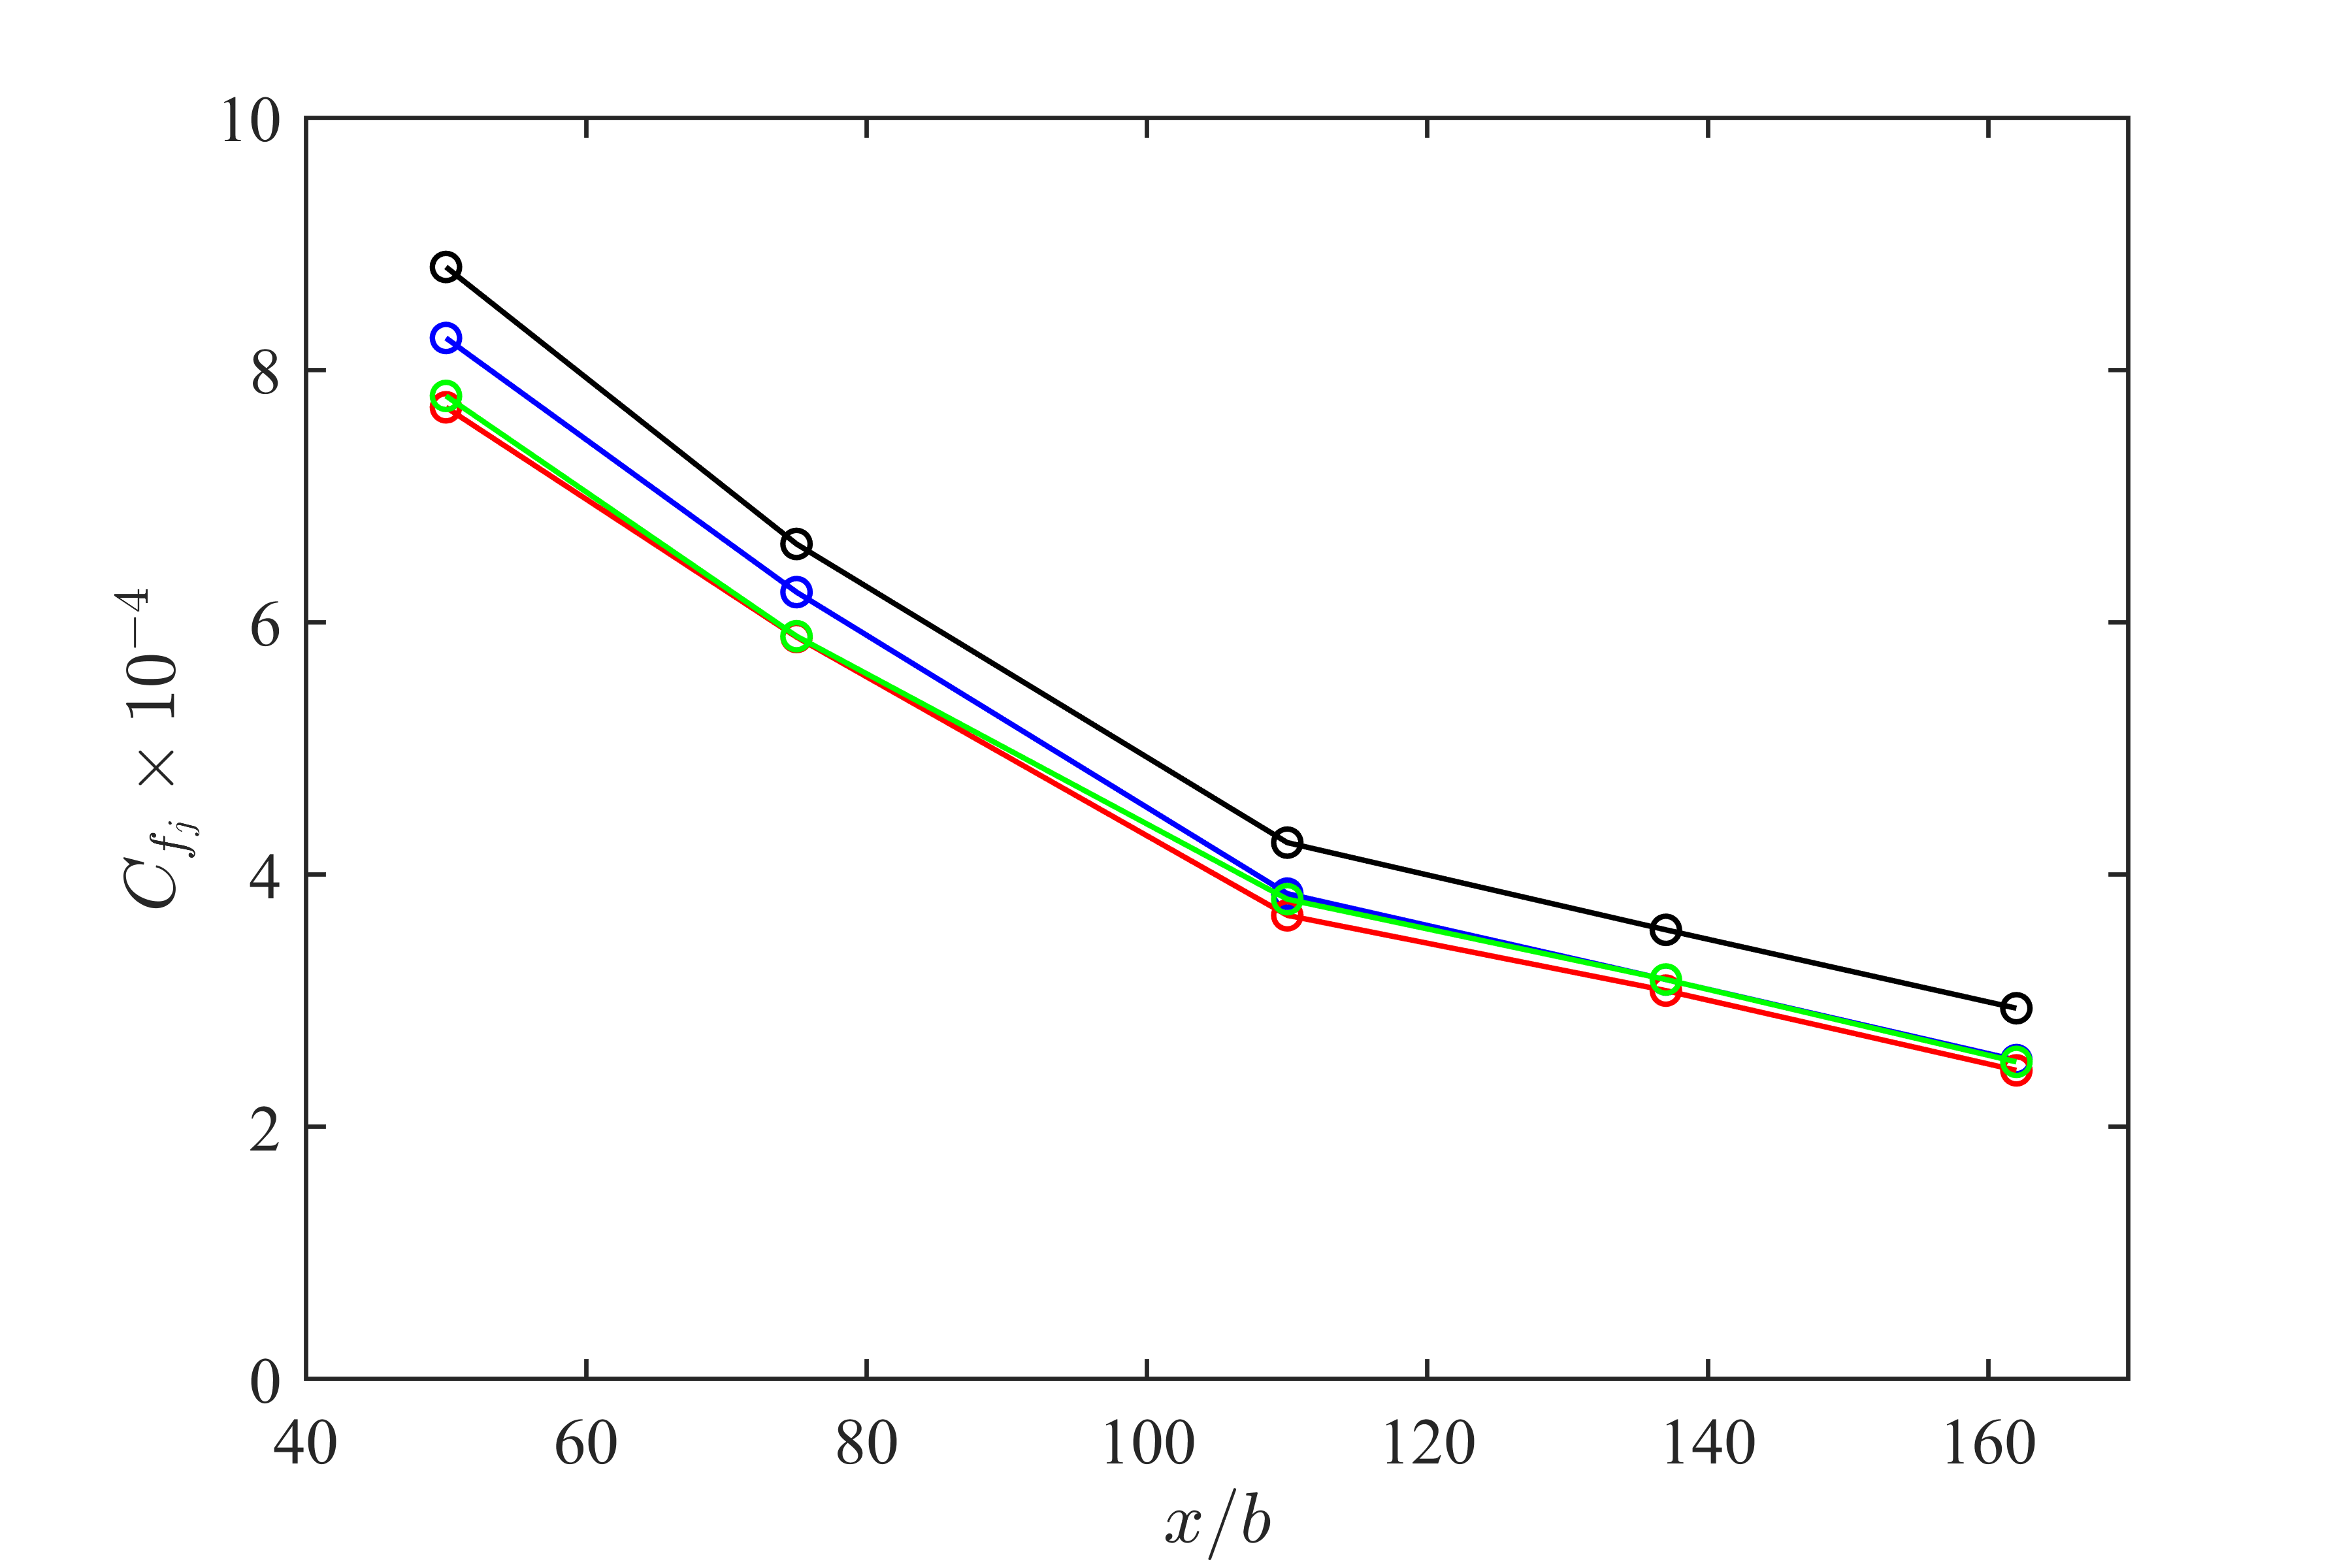
\includegraphics[width=.65\textwidth]{pics/Cfj.png}
	\caption{Skin friction coefficient $C_{f_j} = 2U_{\tau}^2 / V_j^2$ as a function of  streamwise distance $x/b$ for the forced flow. The color convention from Figure~\ref{fg:meanVel137} is followed here.}
	\label{fg:cfj}
\end{figure}


\begin{figure}[h!]
	\centering
	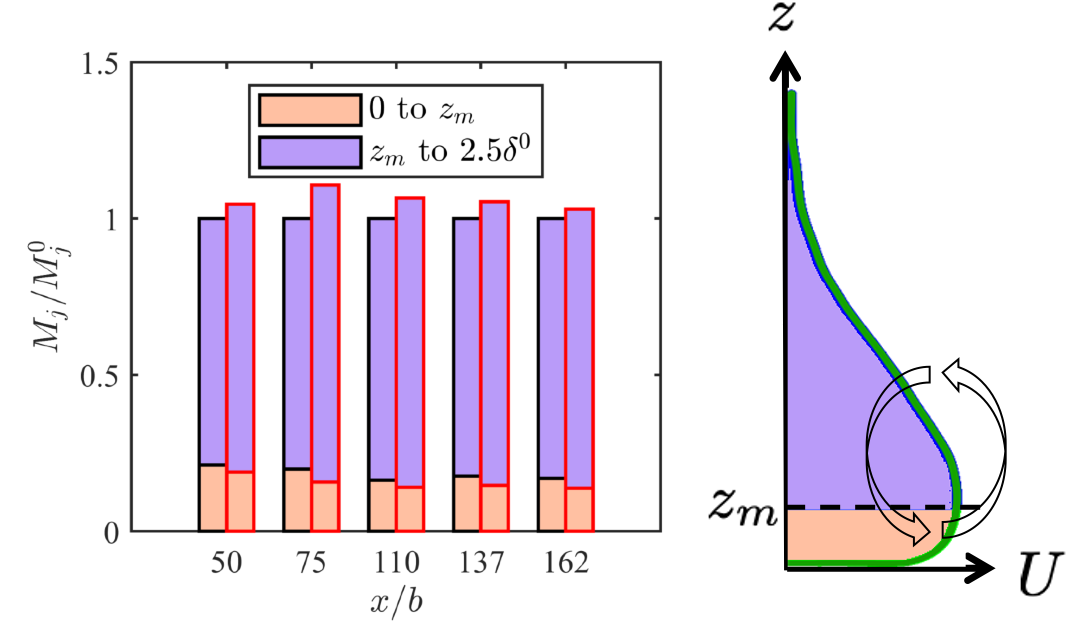
\includegraphics[width=.65\textwidth]{pics/momentum.png}
	\caption{Flow momentum in the inner ($z<z_m$) and outer ($z>z_m$) regions of the flow. The variation is shown as a function of streamwise distance for case A. A schematic highlighting the enhanced mixing in the forced flow is also shown. }
	\label{fg:mom}
\end{figure}

The variation of the skin friction coefficient $C_{f_j} = 2U_{\tau}^2 / V_j^2$ as a function of downstream distance is shown in Figure~\ref{fg:cfj}. The profiles for all three forcing cases are shown. $C_{f_j}$ is seen to decrease upon forcing for all three cases consistent with Figure~\ref{fg:uTauStNum}, the maximum decreases at all streamwise locations being that corresponding to case B. 

The forcing caused changes in the momentum residing in the inner and outer parts of the flow. The momentum in the flow is divided into two parts using a broad division based on wall normal location. The momentum in the flow in the inner wall region ($z<z_m$) and the outer region ($z>z_m$) is shown in Figure~\ref{fg:mom} as function of downstream distance. The overall momentum in the flow is increased by the forcing at all streamwise locations. On the other hand, the momentum in the inner wall region is reduced at all streamwise locations. The increased mixing in the flow upon forcing simultaneously removes high momentum fluid from the wall region while bringing in low momentum fluid from the outer region (see schematic of Figure~\ref{fg:mom}). This decreases the momentum in the wall region which the reduces the mean skin friction coefficient.

\section{Linear Response}

\begin{figure}[h]
	\centering
	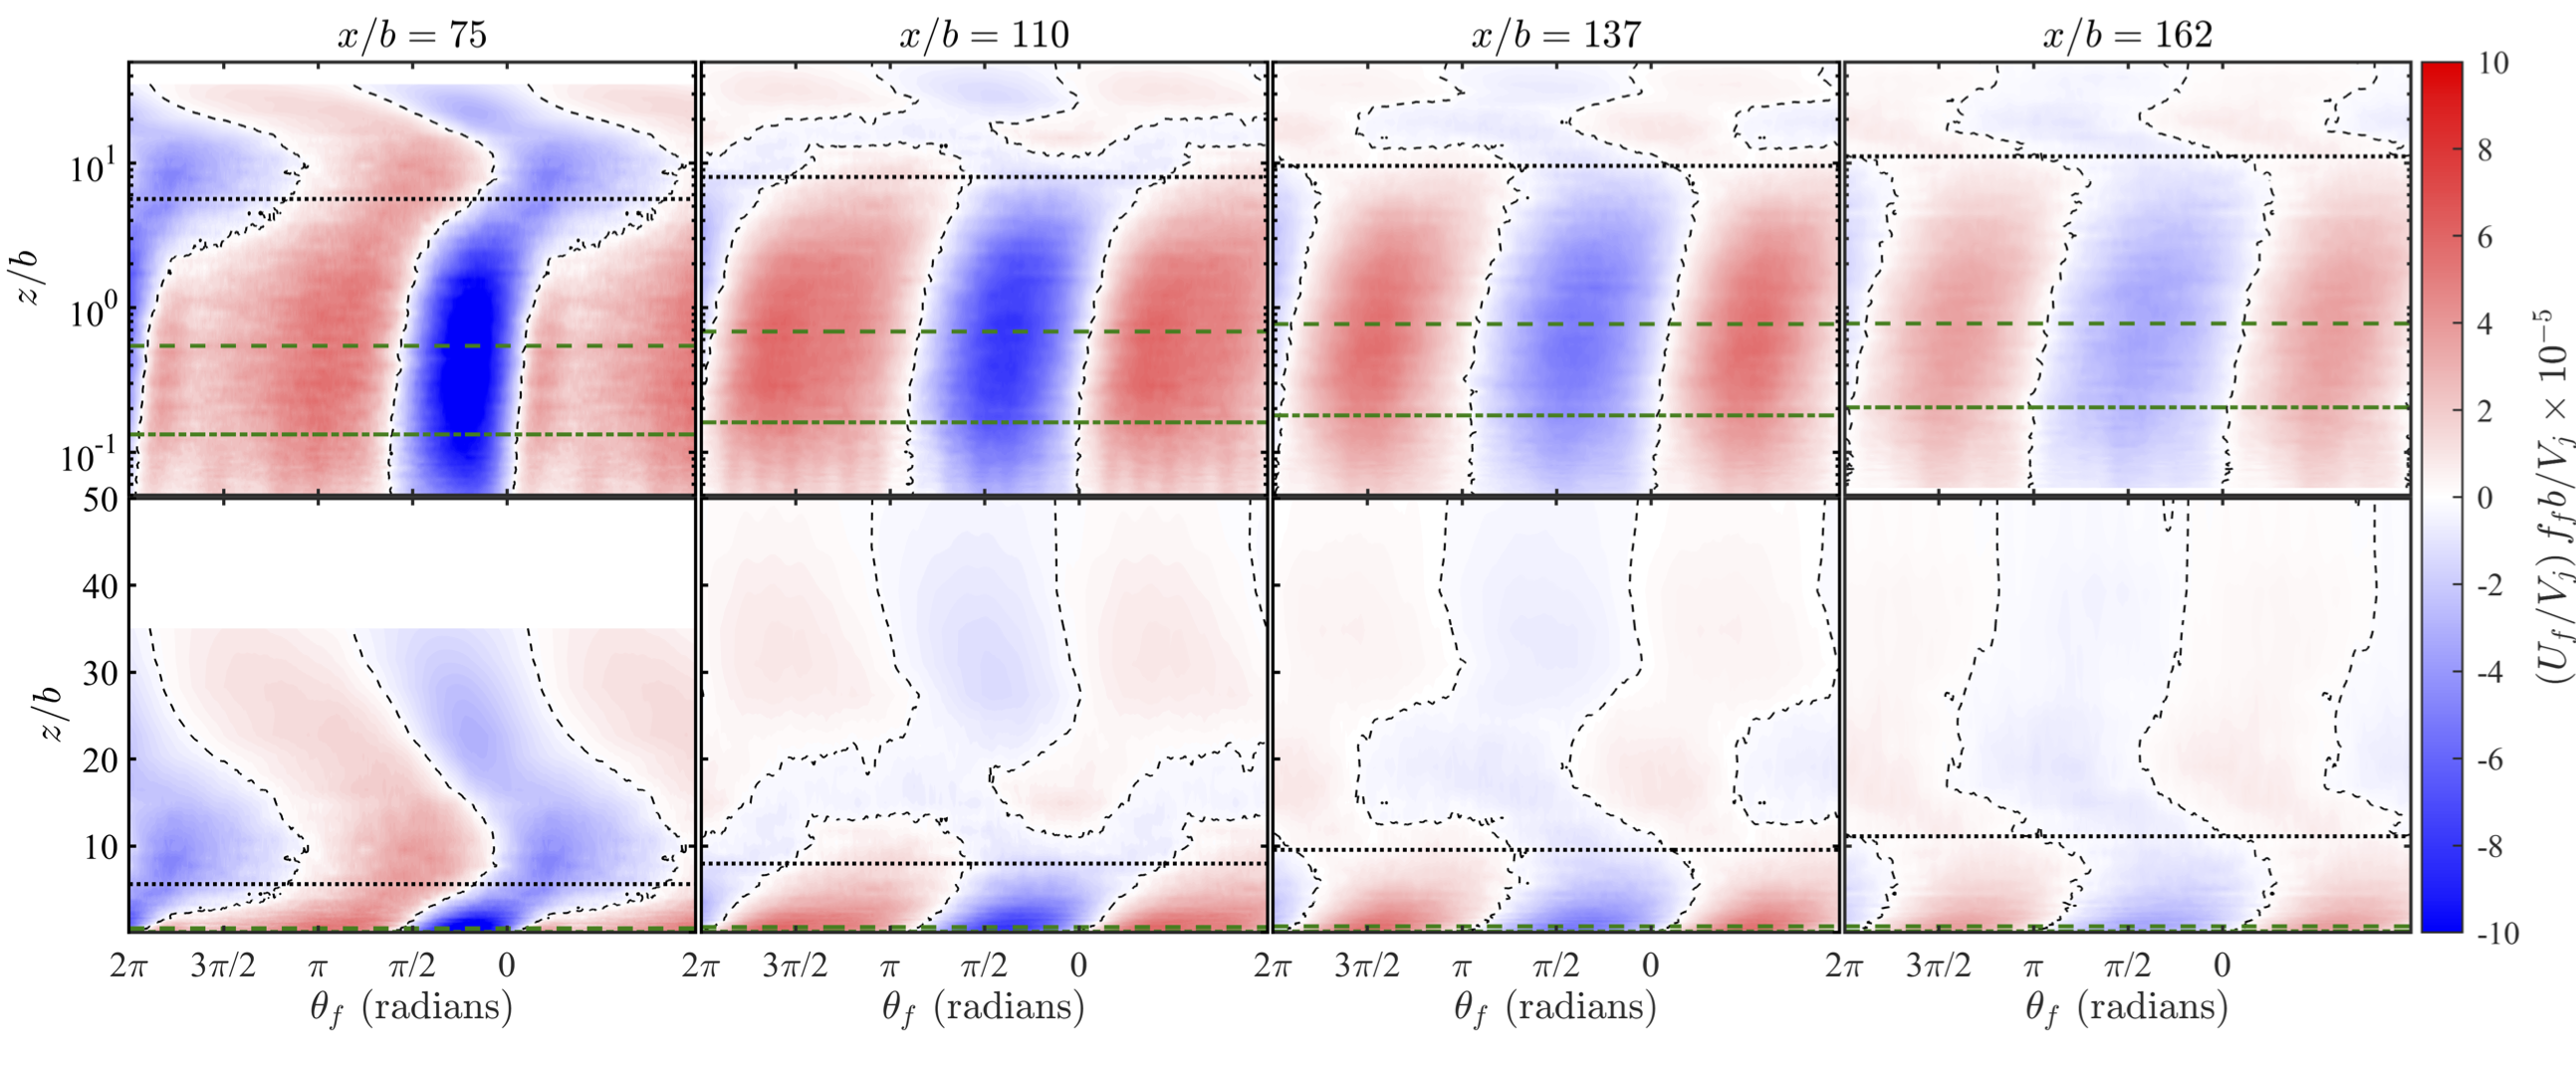
\includegraphics[width=.99\textwidth]{pics/linearResponse.png}
	\caption{Variation of the linear response mode $U_f$ in logarithmic coordinates (top) and linear coordinates (bottom) for case A. The red regions indicate positive fluctuation whereas the blue regions indicate negative fluctuations. The line (\dotted) is that corresponding to $U_f = 0$.}
	\label{fg:linResp}
\end{figure}

\begin{figure}[h]
	\centering
	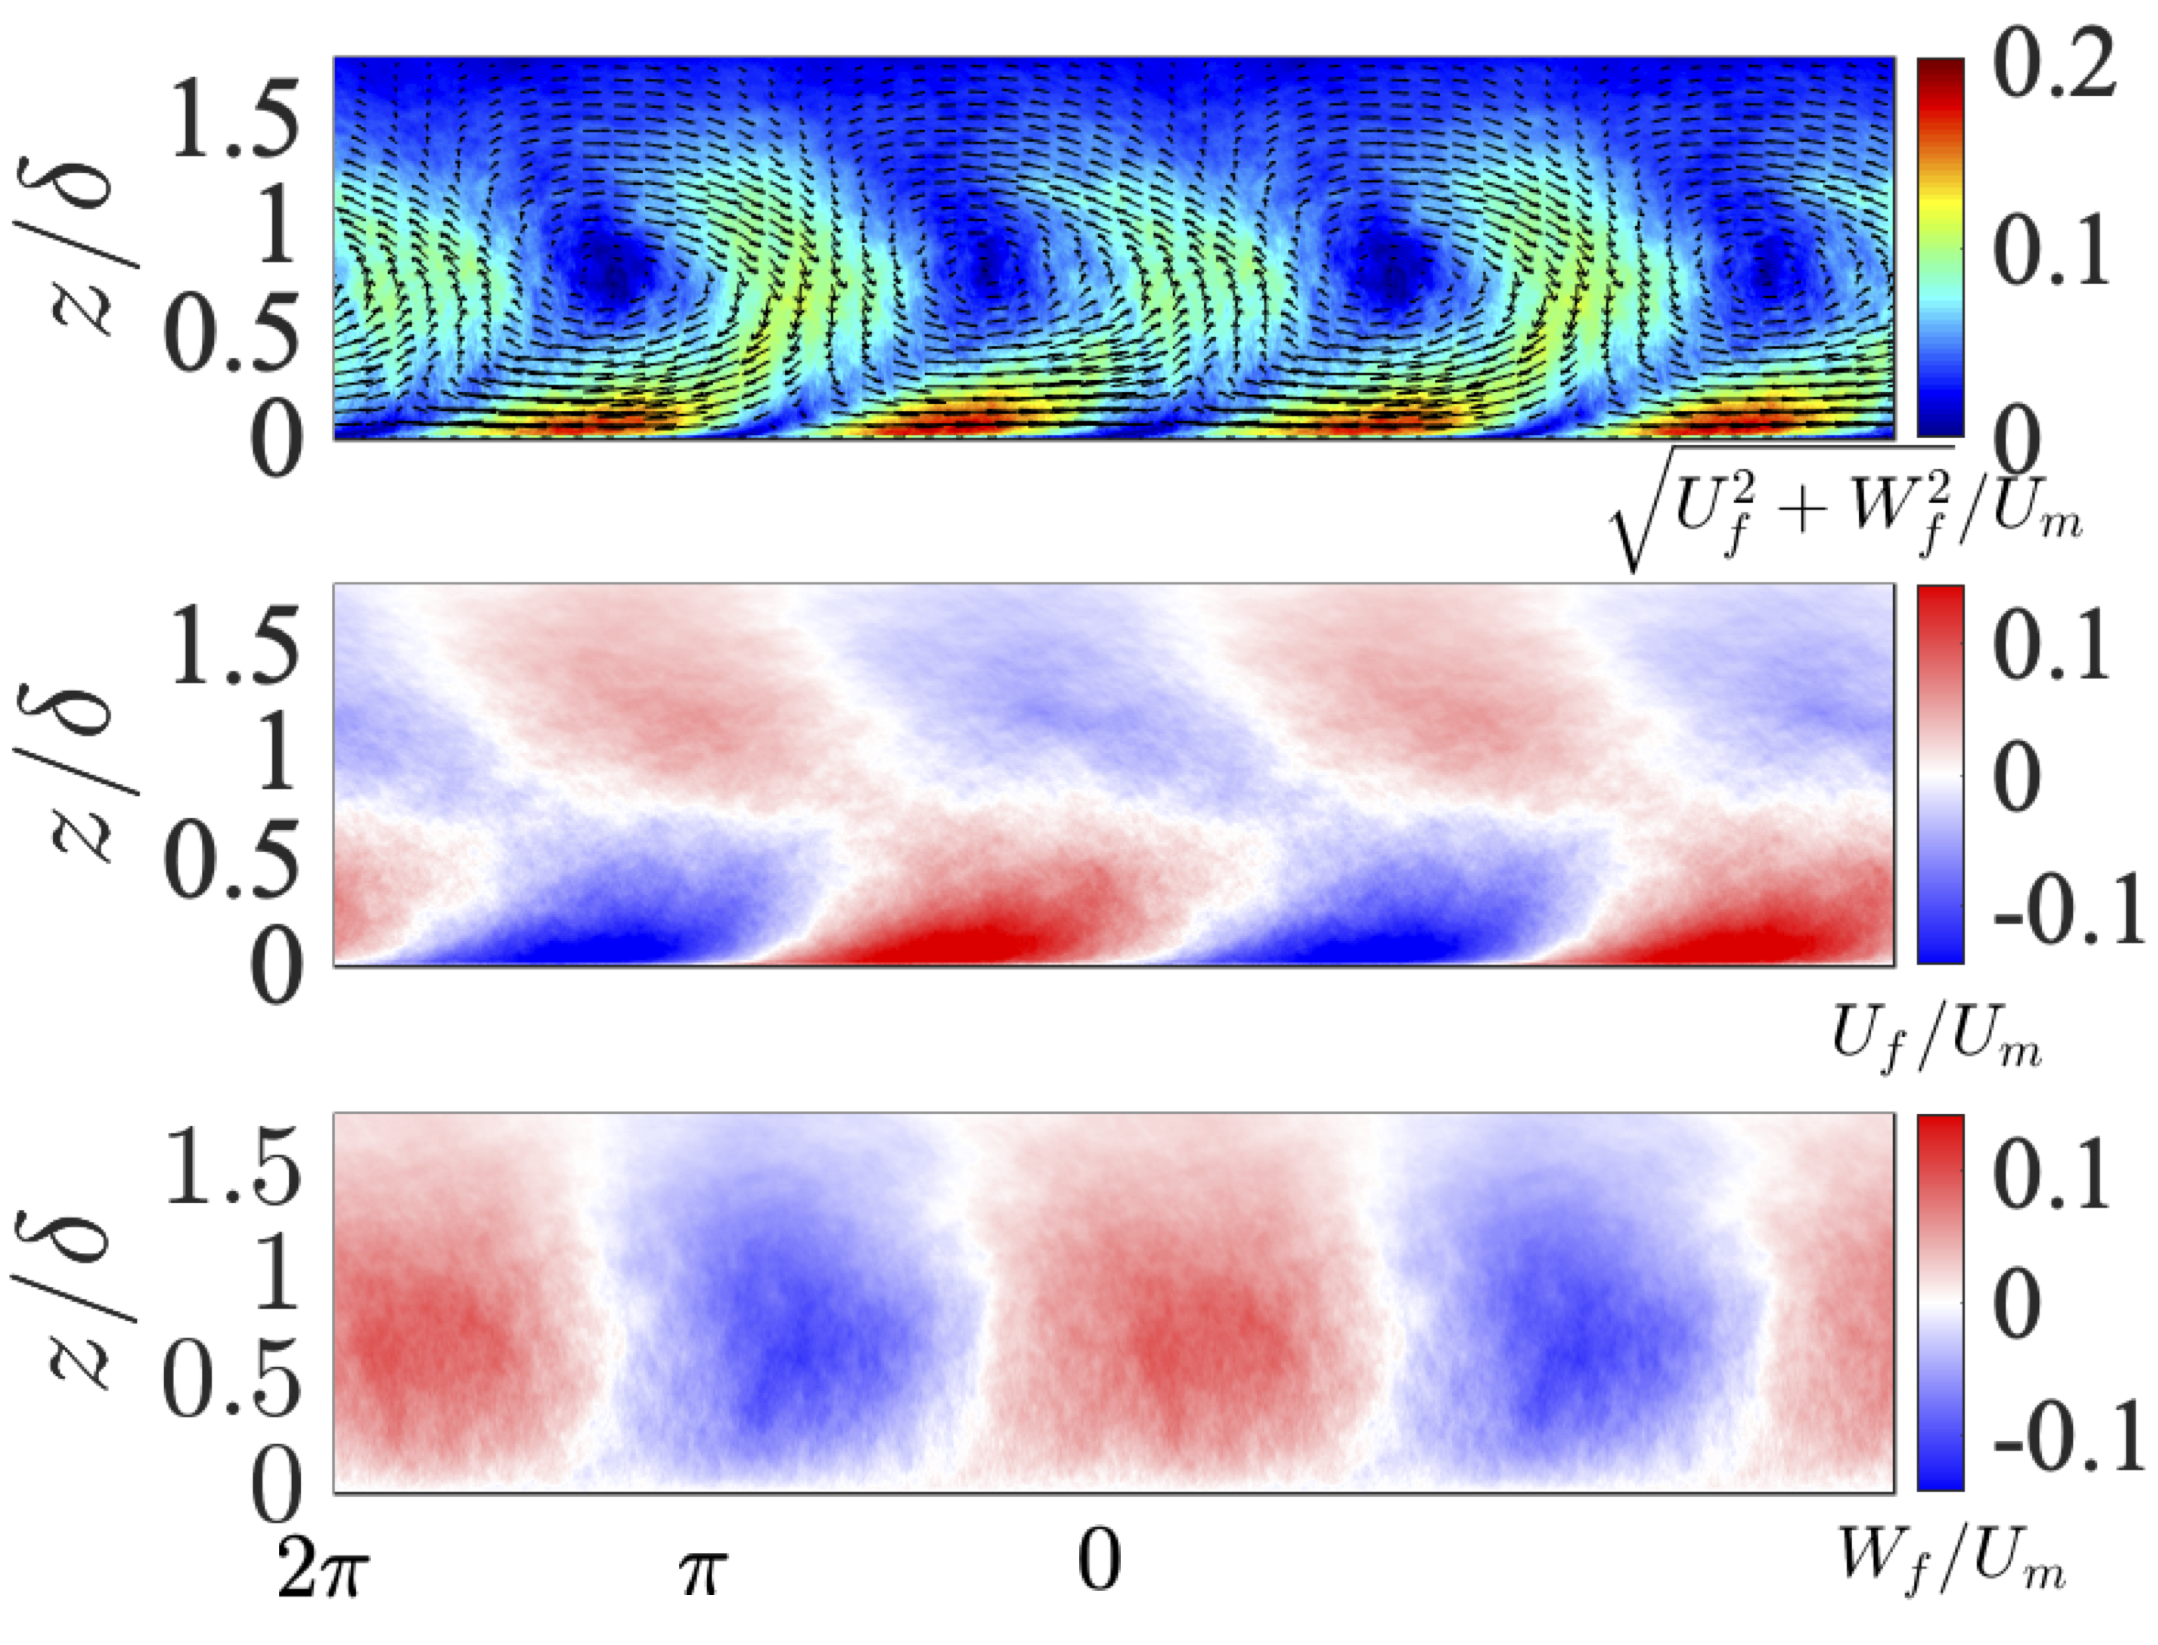
\includegraphics[width=.8\textwidth]{pics/linearResponse137.png}
	\caption{Linear response mode from the PIV based measurements. Both the streamwise $U_f$ (middle) and wall-normal $W_f$ (bottom) component are shown. The velocity vectors corresponding to these modes are also shown (top). }
	\label{fg:linResp137}
\end{figure}

The linear response mode of the PWJ, due to the applied perturbation $U_f(\theta_f,z)$, as a function of downstream distance, is shown for case A in Figure~\ref{fg:linResp}. These response modes were constructed based on phase-locked HWA measurements. At all streamwise locations the response in the wall region is a forward leaning flow structure. This structures is similar to the naturally occurring forward leaning structures observed in canonical boundary layers~\citep{Tutkun2009a}. Such structures have also been observed to naturally occur in the wall region of the PWJ~\citep{Banyassady2014a}. In the outer free-shear region, the linear response mode shows a structure that is backward leaning. Such backward leaning flow structures have also been naturally observed in the outer region of the PWJ ~\citep{Banyassady2014a}. At the most downstream locations where $x/b>110$ the linear response modes appears to show a third structure in the outer reaches of the flow. These linear response modes observed in the forced flow at various wall-normal locations show a relative phase shift between each other as a function of streamwise distance. This indicates that these structures are convecting with different convection velocities.

The linear response mode from the PIV based measurements for case A at $x/b=137$ is shown in Figure~\ref{fg:linResp137}. In this case, both the streamwise $U_f$ and the wall-normal $W_f$ modes are shown along with a vectorial representation of the modes. It is reiterated that the structure in the near-wall region is a forward leaning boundary layer like structure while the outer structure is a back leaning jet like structure. They are together associated with alternating regions of positive and negative wall-normal motions. 

\section{Spectral Response}

\begin{figure}[h!]
	\centering
	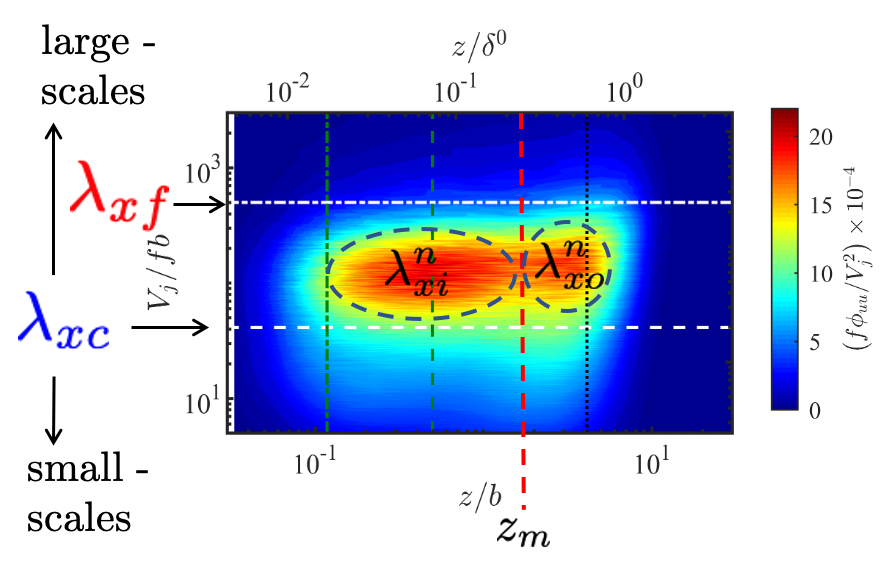
\includegraphics[width=.65\textwidth]{pics/spectra50Unforced.png}
	\caption{Contours of the pre-multiplied one-dimensional energy spectra $f\phi_{uu}$ at $x/b=50$ for the unforced flow. $\lambda_{xf}$ is the forcing wavelength, $\lambda_{xc}$ is the cut-off wavelength that separates the large-scales from the small-scales. $\lambda_{xi}^n$ are the naturally occuring energetic large-scales in the wall (inner) region and $\lambda_{xo}^n$ are the naturally occuring energetic large-scales in the jet (outer) region. The wall-normal locations highlighted are $z^+\approx 15$ (\textcolor{green}{\chain}), $z^+\approx 60$ (\textcolor{green}{\dashed}) and $z\approx 0.6\delta^0$ (\textcolor{black}{\dotted})}
	\label{fg:spec50uf}
\end{figure}

\begin{figure}[h!]
	\centering
	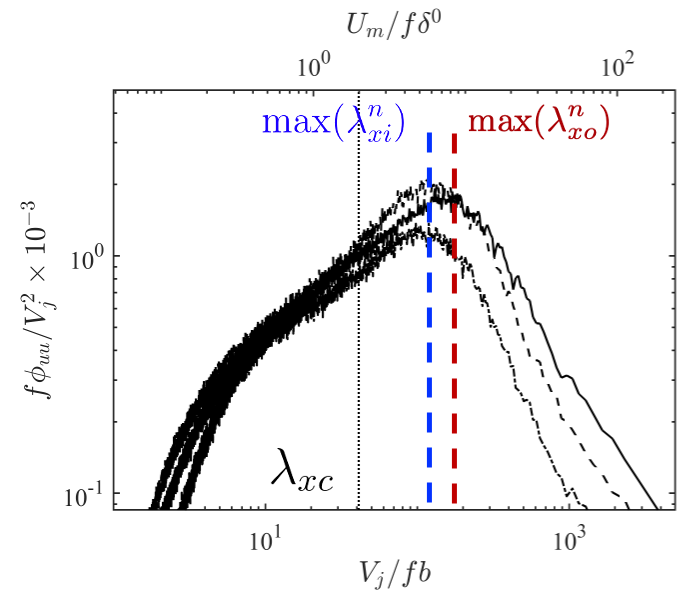
\includegraphics[width=.65\textwidth]{pics/spectra50LineUnforced.png}
	\caption{Profiles of the pre-multiplied one-dimensional energy spectra $f\phi_{uu}$ at $x/b=50$ for the unforced flow showing the wall-normal locations highlighted in Figure~\ref{fg:spec50uf}. The line styles are as follows, $z^+\approx 15$ (\textcolor{black}{\chain}), $z^+\approx 60$ (\textcolor{black}{\dashed}) and $z\approx 0.6\delta^0$ (\textcolor{black}{\full}). Also highlighted are the cutoff wavelength $\lambda_{xc}$ and the most energetic wavelengths in the wall region $\textrm{max}(\lambda_{xi}^n)$ and the outer region $\textrm{max}(\lambda_{xo}^n)$ respectively. }
	\label{fg:spec50lnuf}
\end{figure}

First, the one-dimensional pre-multiplied energy spectra  $f\phi_{uu}$ of the unforced flow is considered to highlight key flow features. Figure.~\ref{fg:spec50uf} shows the spectra $f\phi_{uu}$ of the unforced flow at $x/b=50$. The energy spectra is presented as a function of a wavelength $V_j f/b$ and wall-normal distance $z$, where $f$ are the Fourier frequencies. Shown also is the cut-off wavelength $\lambda_{xc}$ that is used to separate the large-scales from the small-scales. Here, large-scales refers to those flow scales that are larger than twice the outer length scale of the unforced flow i.e., $\lambda_x> 2\delta^0$. The profiles of the spectra $f\phi_{uu}$ at three wall-normal locations ($z^+\approx 15,~60$ and $z\approx 0.6\delta^0$) are shown in Figure~\ref{fg:spec50lnuf}. These locations are chosen to represent the very-near wall region, a location in the log region and one in the outer jet region respectively. Much of the energy in the unforced PWJ resides in the large-scales of the flow. There are however two wall-normal locations where this energy is concentrated. One lies in the inner wall region centered around the wall-normal location $z^+\approx 60$ and the other is in the outer jet region centered around the wall-normal location $z\approx 0.6\delta^0$. These energetic large-scale wavelengths are referred to as $\lambda_{xi}^n$ and $\lambda_{xo}^n$ respectively. Here, the superscript $n$ is used to highlight that these are naturally occurring. Each of these group of energetic large-scale wavelengths $\lambda_{xi}^n$ and $\lambda_{xo}^n$ have a wavelength with maximum or peak energy and is referred to as $\textrm{max}\left(\lambda_{xi}^n\right)$ or $\textrm{max}\left(\lambda_{xo}^n\right)$ respectively. It is also noted that $\textrm{max}\left(\lambda_{xi}^n\right) < \textrm{max}\left(\lambda_{xo}^n\right)$ (see Figure~\ref{fg:spec50lnuf}).



\begin{figure}[h!]
	\centering
	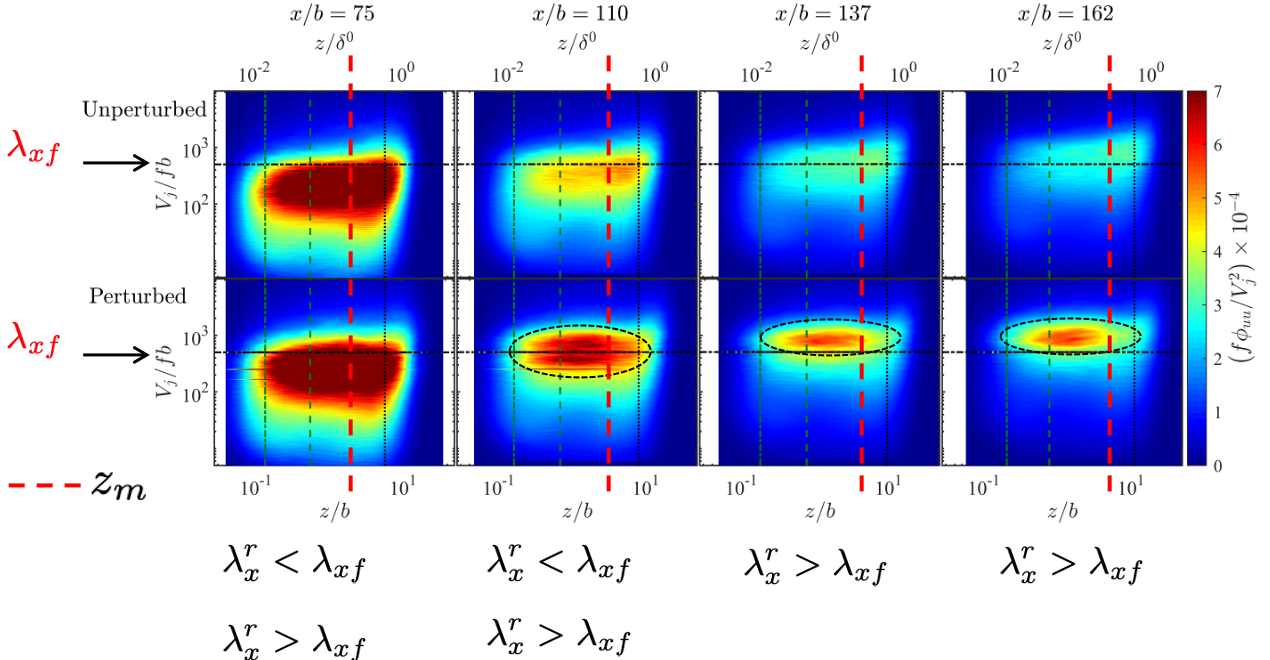
\includegraphics[width=.99\textwidth]{pics/specEvol.png}
	\caption{Streamwise evolution of the contours of the energy spectra $f\phi_{uu}$ for the unforced (top) and forced (bottom) flow (case A). The forcing scale $\lambda_{xf}$ is also shown. The relative size of the forcing scale $\lambda_{xf}$ to the recipient scales $\lambda_x^r$ are indicated below the plots. The recipient scales $\lambda_x^r$ in the forced spectra are highlighted over the contours (\dashed).}
	\label{fg:specEvol}
\end{figure}

The streamwise evolution of the energy spectra $f\phi_{uu}$ of the unforced flow and the forced flow is shown in Figure~\ref{fg:specEvol}. The forced flow spectra shown is that corresponding to case A. As the unforced flow develops downstream the energetic large-scales of the flow become larger with increasing downstream location i.e., $\lambda_{xi}^n$ and $\lambda_{xo}^n$ increase with $x/b$. However, the forcing wavelength $\lambda_{xf}$ is fixed. Therefore, at the most upstream locations ($x/b\leq 110$) $\lambda_{xf}>\lambda_{xo}^n>\lambda_{xi}^n$. At a downstream location of $x/b\approx 110-137$, $\lambda_{xf}\approx \mathrm{max}\left(\lambda_{xo}^n\right)$. At further downstream locations $\lambda_{xf}<\lambda_{xi}^n<\lambda_{xo}^n$. 

\begin{figure}[h!]
	\centering
	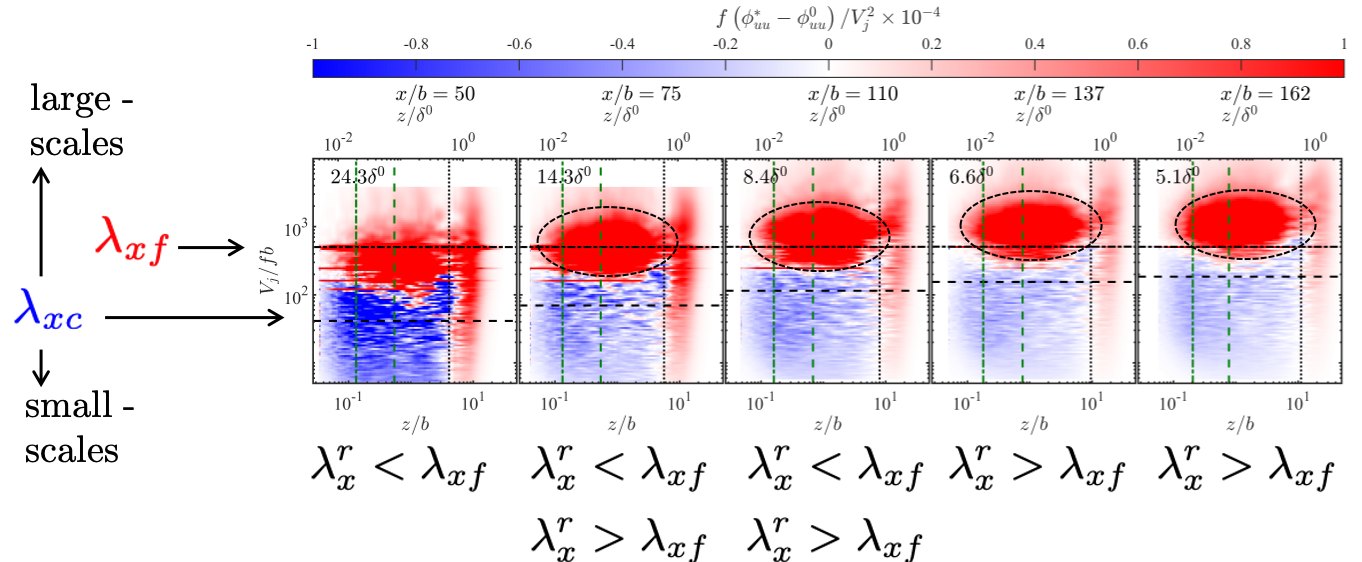
\includegraphics[width=.99\textwidth]{pics/specEvol2.png}
	\caption{Streamwise evolution of the contours of the difference in the energy spectra $f(\phi_{uu}^*-\phi_{uu})$ between the forced (case A) and the unforced flow. The forcing scale $\lambda_{xf}$ as well as the cutoff wavelength $\lambda_{xc}$ are also shown. The relative size of the forcing scale $\lambda_{xf}$ to the recipient scales $\lambda_x^r$ are indicated below the plots. The recipient scales $\lambda_x^r$  in the forced spectra are highlighted over the contours (\dashed). The wall-normal locations highlighted are $z^+\approx 15$ (\textcolor{green}{\chain}), $z^+\approx 60$ (\textcolor{green}{\dashed}) and $z\approx 0.6\delta^0$ (\textcolor{black}{\dotted})}
	\label{fg:specEvol2}
\end{figure}


\begin{figure}[h!]
	\centering
	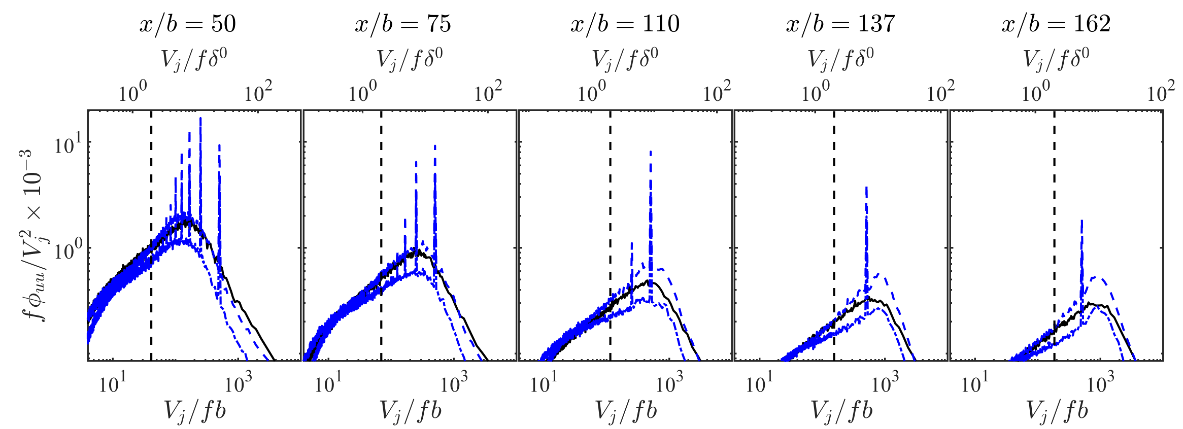
\includegraphics[width=.99\textwidth]{pics/specEvol4.png}
	\caption{Compares the profiles of the pre-multiplied energy spectra of the forced flow (case A)  at the wall-normal locations $z^+\approx 60$ (\textcolor{blue}{\chain}) and $z^+\approx 60$ (\textcolor{blue}{\dashed}). Also shown is the profile of the spectra of the unforced flow at $z\approx 0.6 \delta^0$. These profiles are shown at various streamwise locations.}
	\label{fg:specEvol4}
\end{figure}

\begin{figure}[h!]
	\centering
	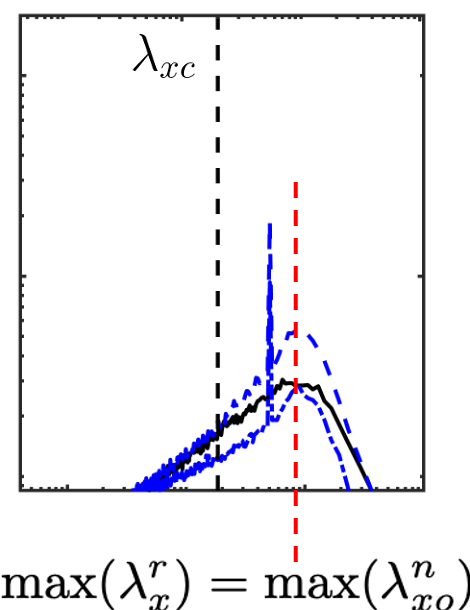
\includegraphics[width=.35\textwidth]{pics/specEvol4_162.png} \vspace{5pt}
	\caption{Compares the profiles of the pre-multiplied energy spectra at $x/b=162$ of the forced flow (case A) at the wall-normal locations $z^+\approx 60$ (\textcolor{blue}{\chain}) and $z^+\approx 60$ (\textcolor{blue}{\dashed}). Also shown is the profile of the spectra of the unforced flow at $z\approx 0.6 \delta^0$. }
	\label{fg:specEvol4_162}
\end{figure}

Considering the forced spectra it is shown that the excess energy is always transferred to the inner wall region, the region that is occupied by the scales $\lambda_{xi}^n$. This is highlighted in the difference plot of Figure~\ref{fg:specEvol2}, where the difference in spectra of the forced and unforced flow are shown as a function of streamwise distance. However, the recipient wavelengths $\lambda_x^r$ of the excess perturbation energy are such that $\mathrm{max} \left(\lambda_{x}^r \right) \approx \mathrm{max}\left(\lambda_{xo}^n\right)$. In other words, the perturbation energy is transferred to a fixed set of scales $\lambda_{xr} \approx \lambda_{xo}^n$ at a fixed wall-normal location, the wall region. This is further highlighted in the line plots of Figure~\ref{fg:specEvol4}. Here the profiles of the pre-multiplied energy spectra of the forced flow (case A) in the wall region ($z^+\approx 15$ and 60) are compared with that of the unforced flow at $z\approx 0.6 \delta^0$. For clarity, these profiles at $x/b=162$ are shown in Figure~\ref{fg:specEvol4_162}. These figure show that the wavelength corresponding to the most energetic recipient scales align with those of the naturally occurring structures in the outer jet region i.e., max($\lambda_x^r\approx$ max($\lambda_{xo}^r$).   

Figure~\ref{fg:specEvol} and \ref{fg:specEvol2} also shows the relative size of the recipient scales $\lambda_x^r$ and the forcing scale $\lambda_x^f$. At the upstream locations when $\lambda_{x}^r<\lambda_{xf}$ the direction of energy transfer is in the manner of a forward cascade while at the downstream locations when $\lambda_{x}^r>\lambda_{xf}$ the energy transfer is in the manner of an inverse cascade. Figure~\ref{fg:specEvol2} also shows that the energy in the small scales are consistently reduced everywhere in the wall region. However, in the far extremities of the flow $z>0.6 \delta^0$, there is an increase in the small scale energy. 

\begin{figure}[h]
	\centering
	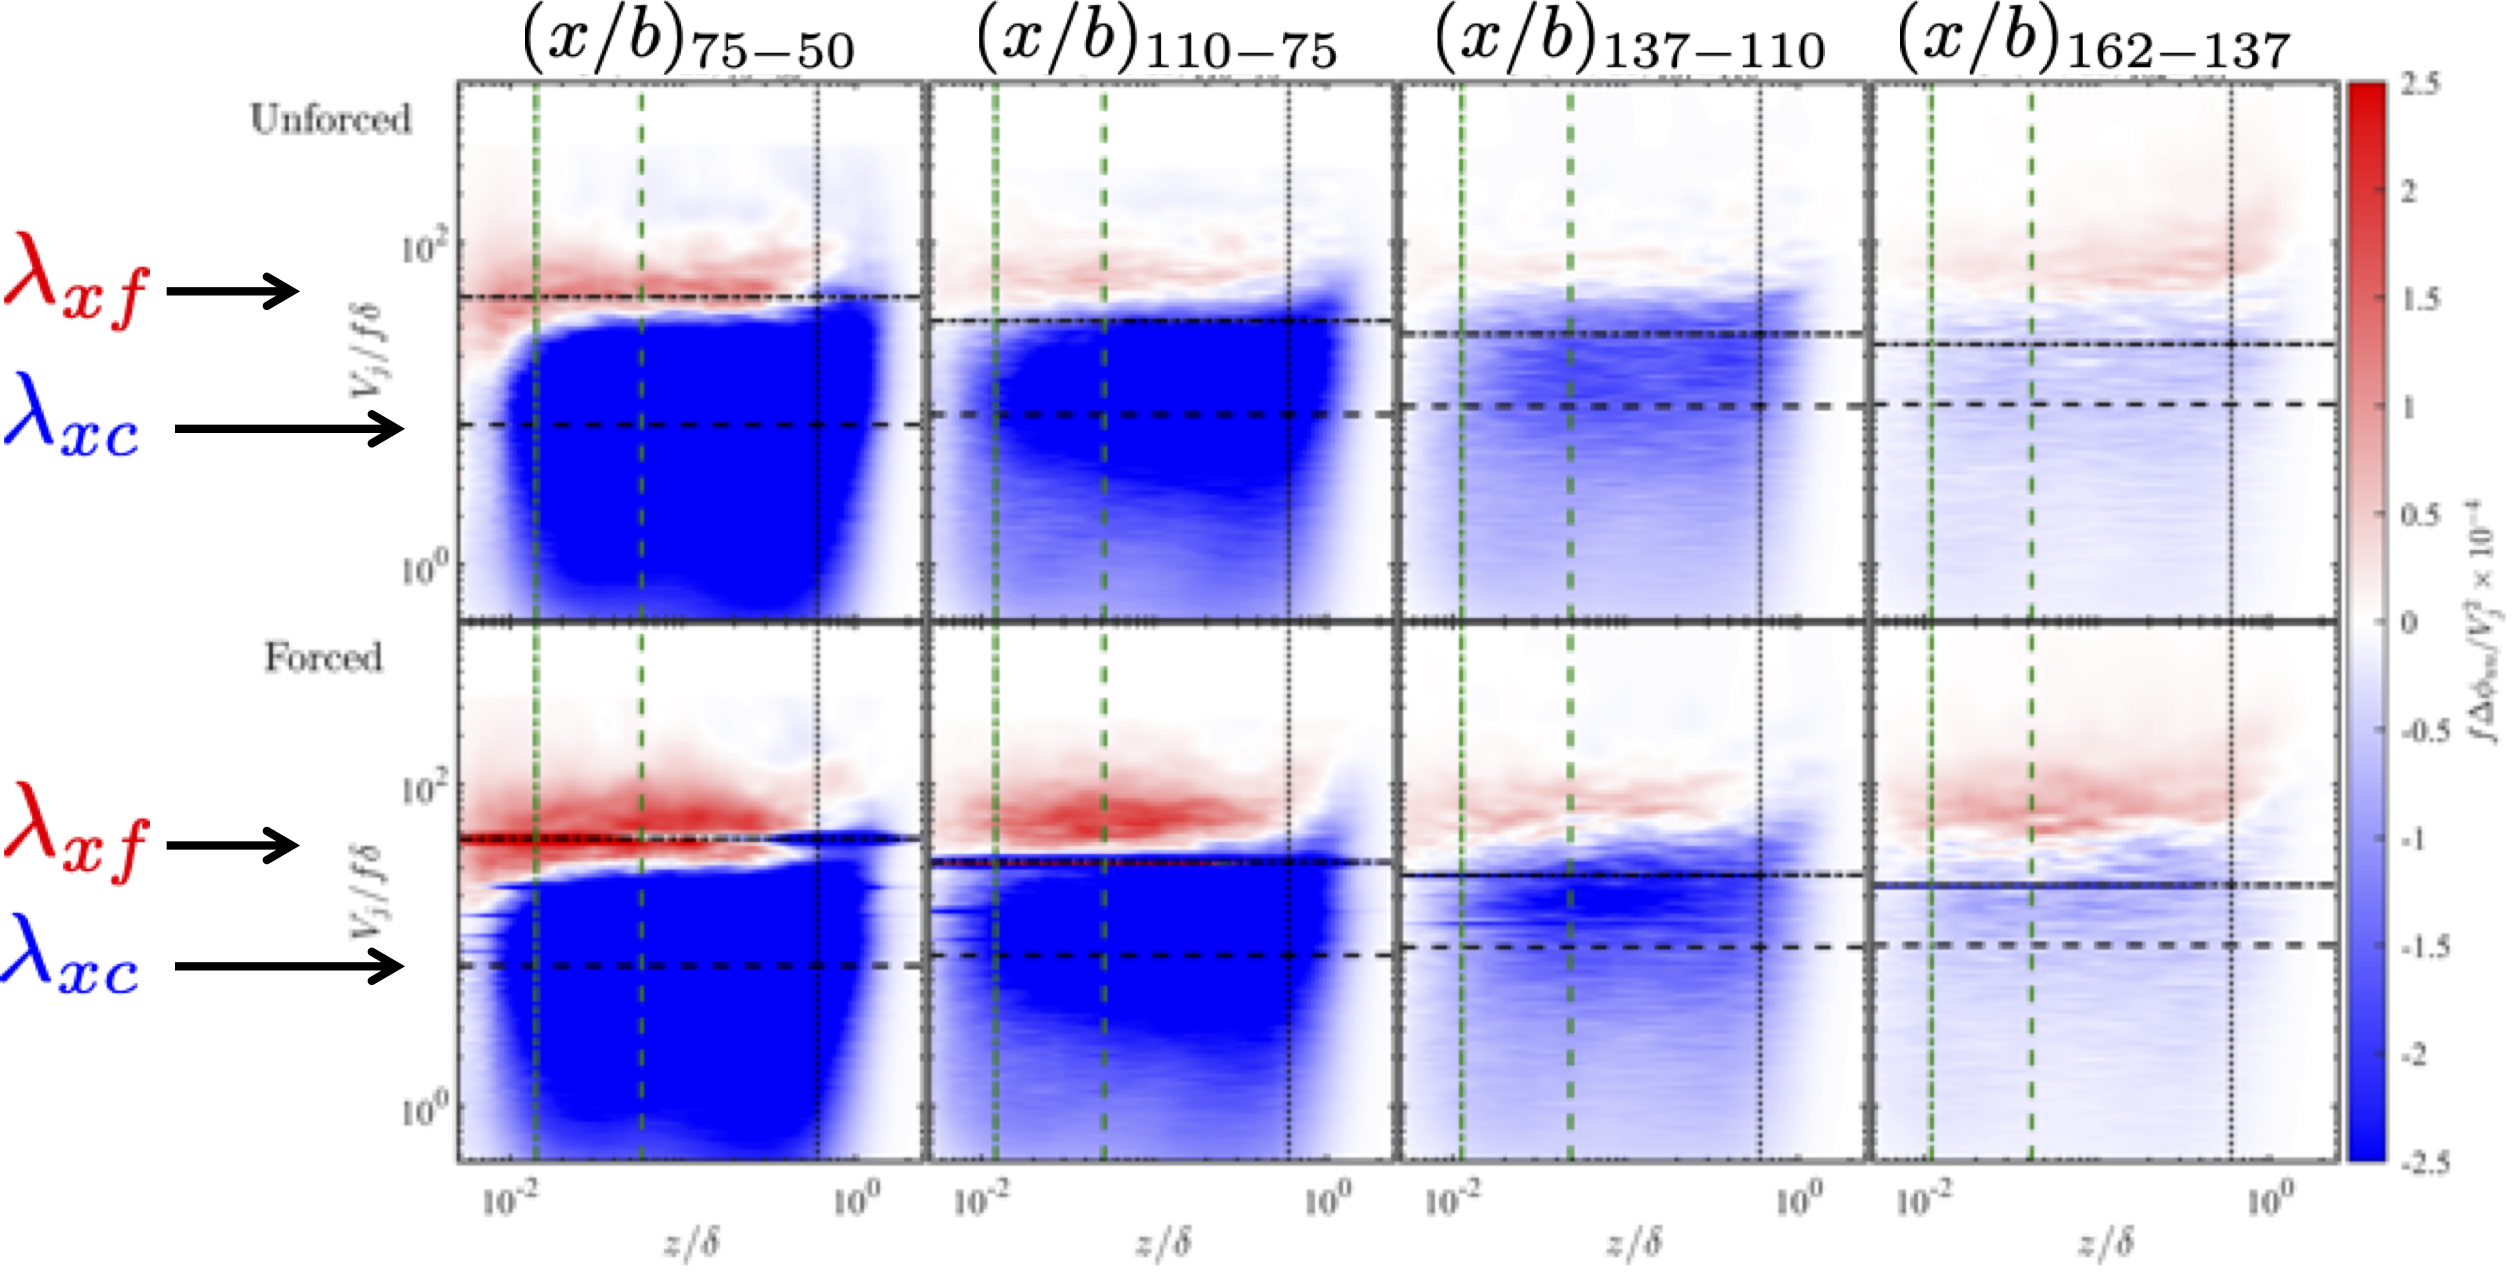
\includegraphics[width=.9\textwidth]{pics/specEvol3.png}
	\caption{Streamwise evolution of the contours of the difference in the energy spectra $f\Delta \phi_{uu}$ between a given streamwise location and the immediately preceding streamwise location. This is shown for both the unforced (top) and the forced (bottom) flow (case A). The forcing scale $\lambda_{xf}$ as well as the cutoff wavelength $\lambda_{xc}$ are also shown. The wall-normal locations highlighted are $z^+\approx 15$ (\textcolor{green}{\chain}), $z^+\approx 60$ (\textcolor{green}{\dashed}) and $z\approx 0.6\delta^0$ (\textcolor{black}{\dotted})}
	\label{fg:specEvol3}
\end{figure}

Figure~\ref{fg:specEvol3} shows the difference in the spectra between that at a given streamwise location and the immediately preceding streamwise location. This is shown for both the forced and unforced flow. This difference plot gives an estimate of the relative energy transfer between scales as the flow develops downstream. The scales that are loosing energy and the scales that are receiving energy as the unforced PWJ develops downstream are exactly the same as the ones that are receiving or loosing energy in the forced PWJ. This of course is except at the forcing frequency and its harmonics in the case of the forced PWJ. This suggests that the mechanisms that exist in the unforced flow are identical to those in the forced flow. Or stated differently, the forcing scale mimics the naturally occurring large-scale structures in the PWJ that occur at the forcing wavelength. 



\begin{sidewaysfigure}[h]
	\centering
	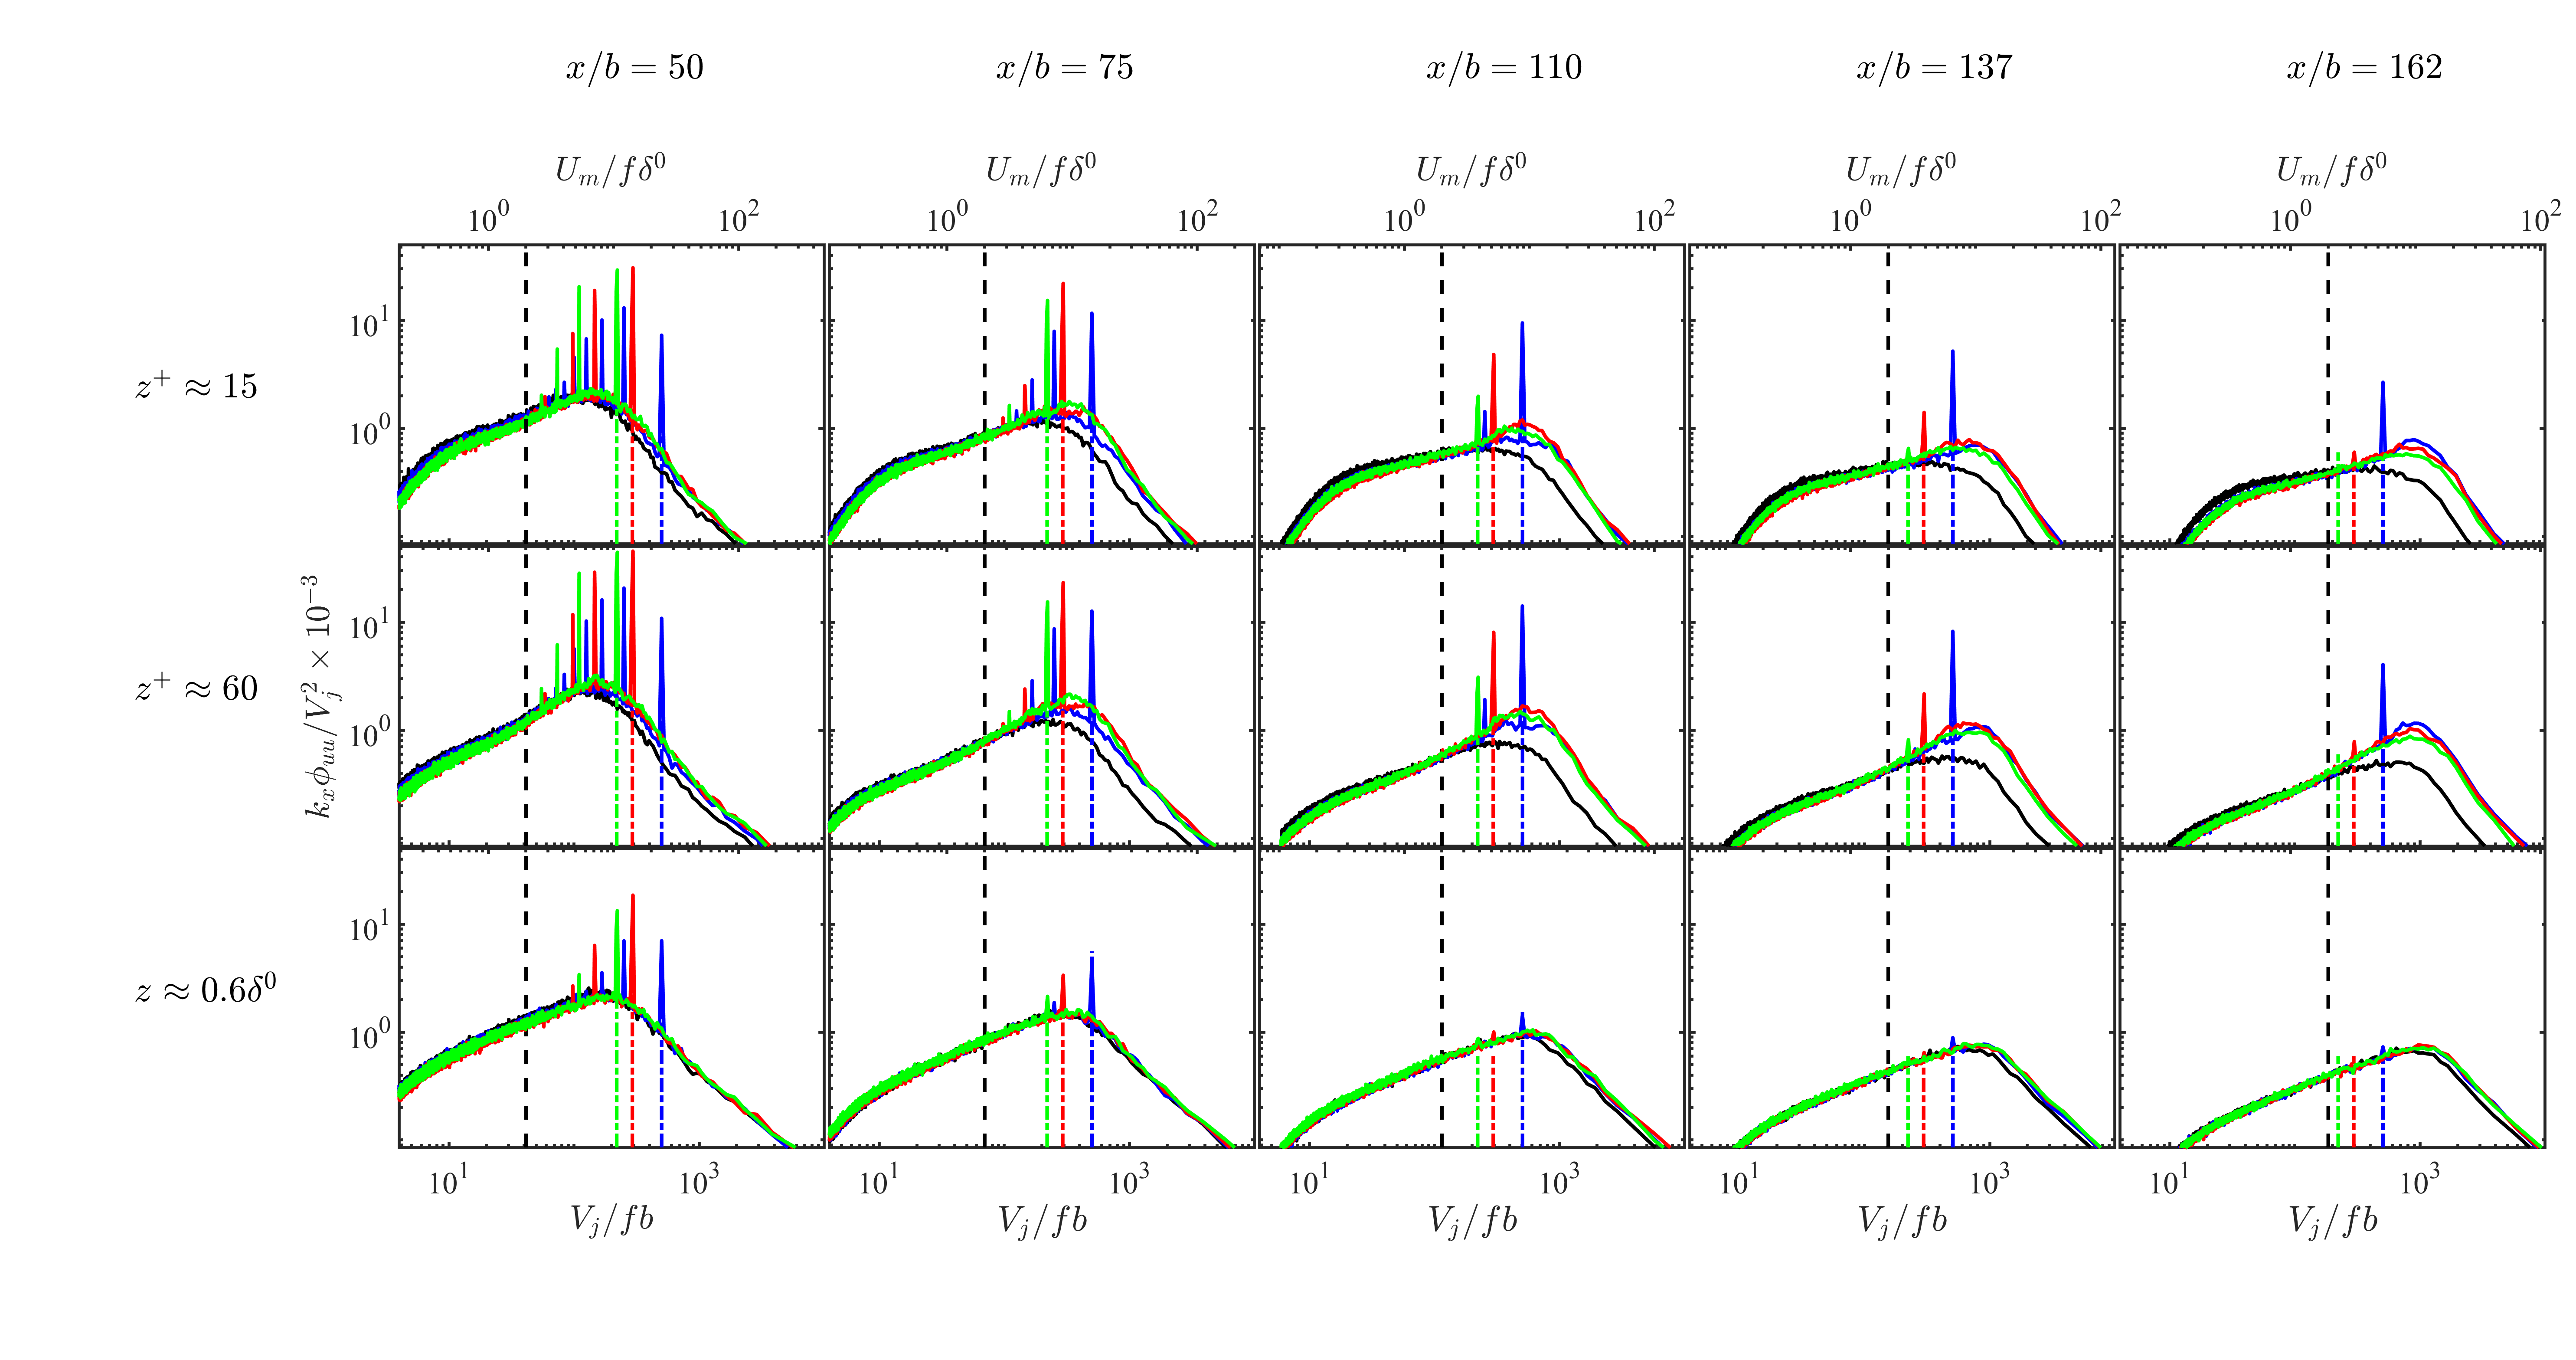
\includegraphics[width=0.99\textwidth]{pics/specLineAll.png}
	\caption{Profiles of the pre-multiplied energy spectra for the unforced (\full) and forced flow; case A (\textcolor{blue}{\full}), case B (\textcolor{red}{\full}) and case C (\textcolor{green}{\full}). The profiles are shown at three wall-normal locations $z^+\approx 15$ (top), $z^+\approx 60$ (middle) and $z\approx 0.6 \delta^0$ (bottom). The forcing scales for the three cases are also shown (dash-dot lines) as well as the cut off wavelength $\lambda_{xc}$ (\dashed).}
	\label{fg:specLnAll}
\end{sidewaysfigure}

This behavior is true for all cases (A, B and C) studied in depth. Figure~\ref{fg:specLnAll} shows the profiles of the pre-multiplied energy spectra for the unforced and forced flow (cases A, B and C). The profiles are shown at three wall-normal locations, two in the inner wall region at $z^+\approx 15$ and 60 and the other in the outer jet region at $z\approx 0.6 \delta^0$. For all the cases the recipient wavelengths $\lambda_x^r$ have a peak energy which occurs at approximately the same wavelength i.e., max($\lambda_x^r$) is identical for all cases. In other words for all the scales of forcing considered, energy from the linear response modes in the near-wall region is being transferred to the outer jet scales. But this energy transfer occurs in the wall region. Also seen is that the small-scale energy for all the forcing scales considered is reduced in the wall region. The linear response mode also persists for longer streamwise distances in the wall region than in the outer region.

\clearpage

\section{Scale Interactions}

\begin{figure}[h!]
	\centering
	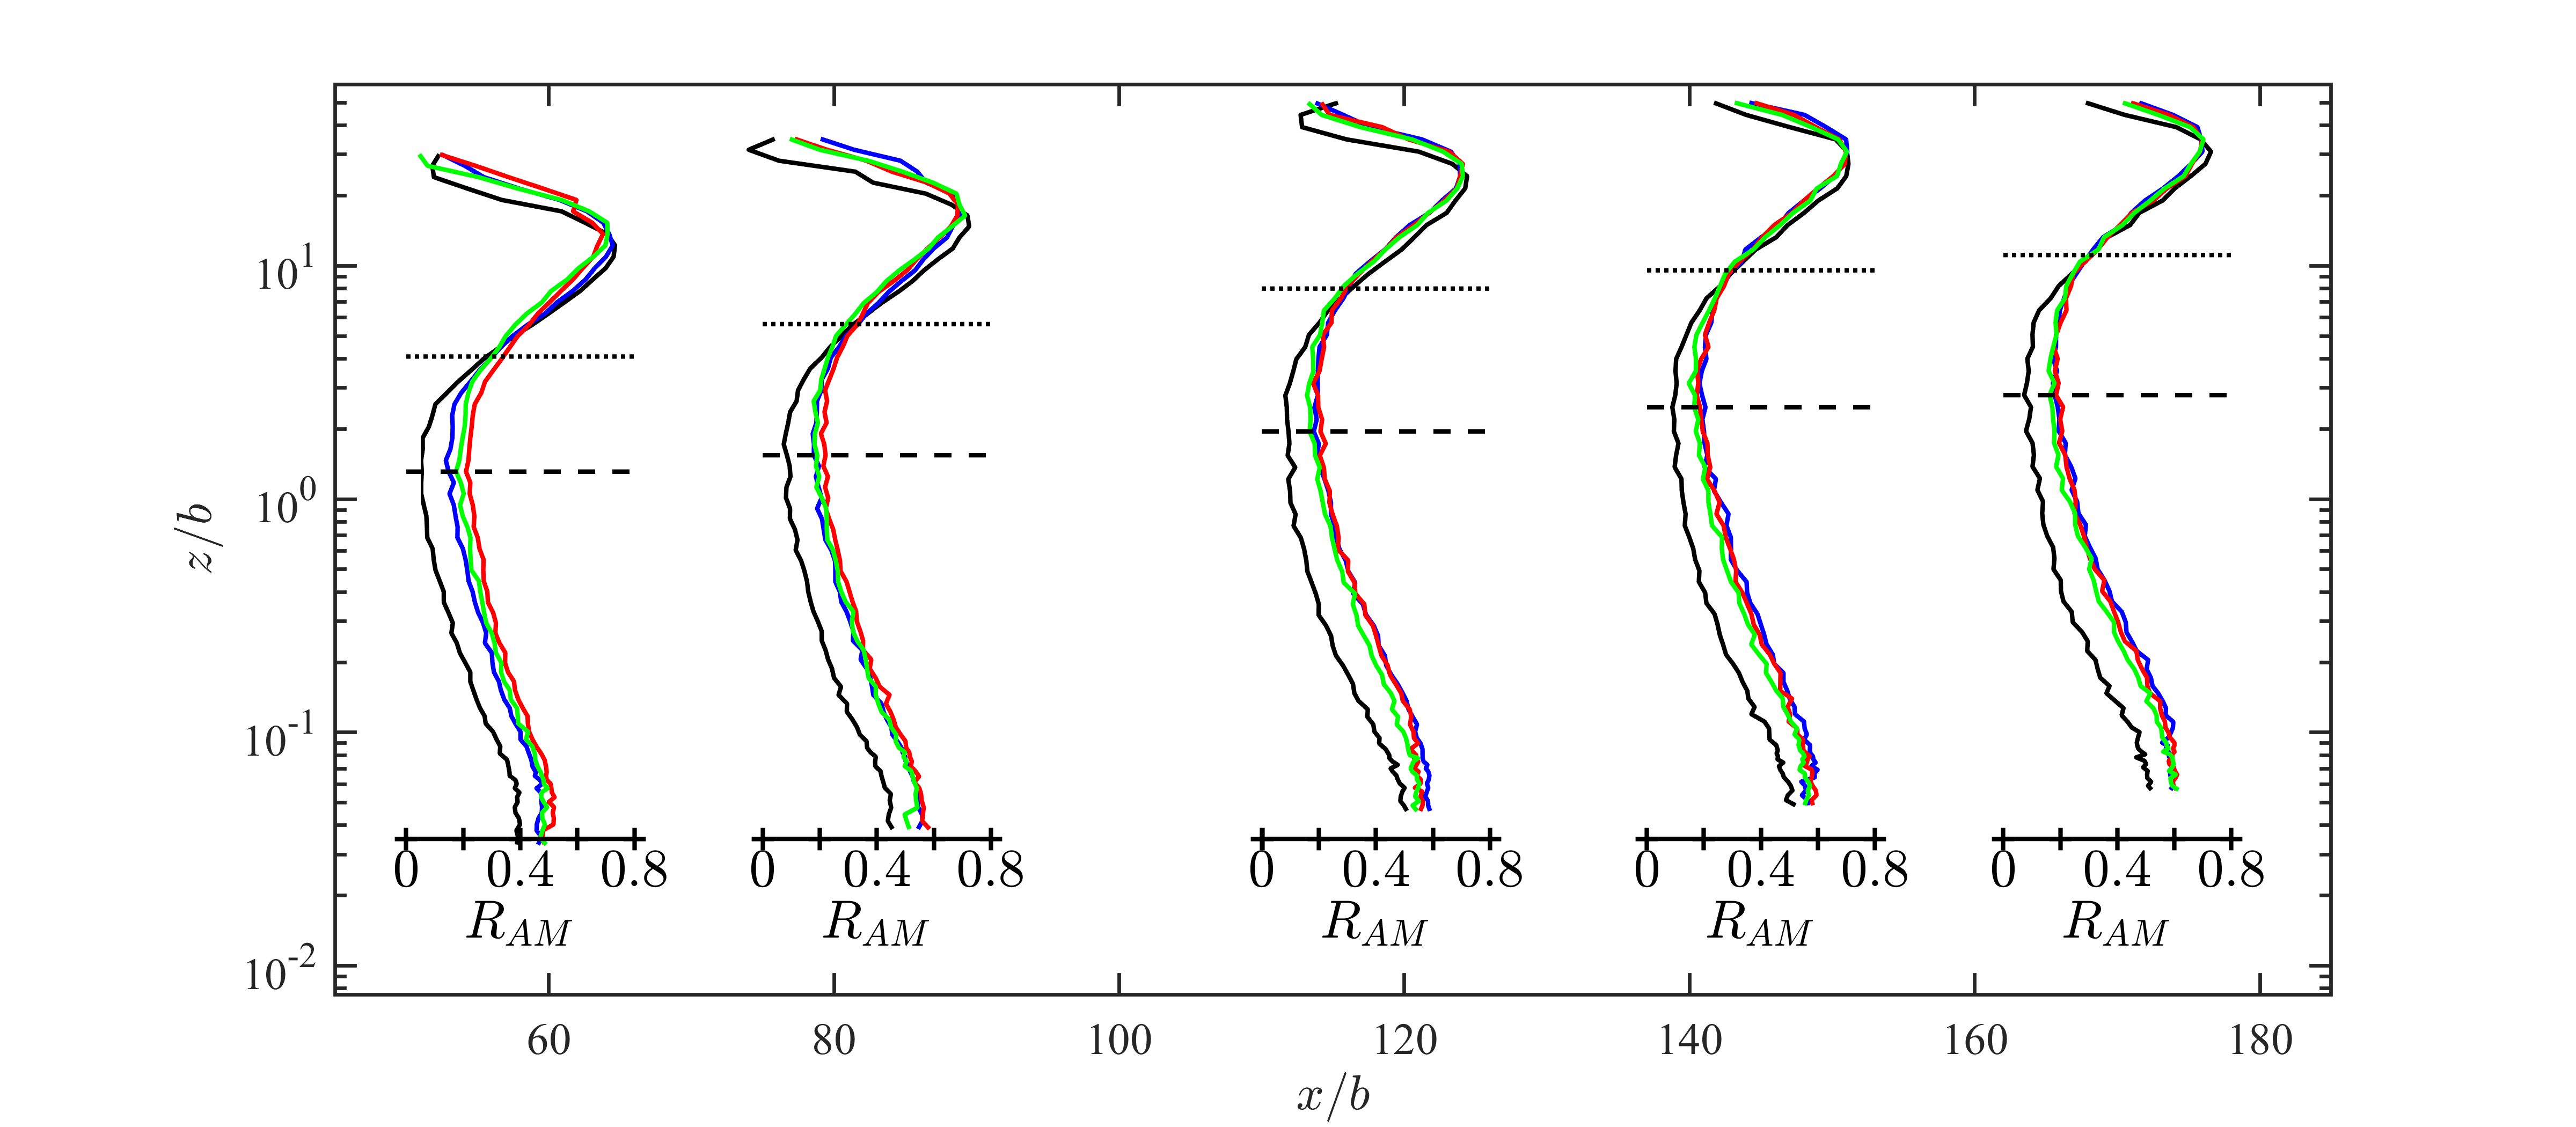
\includegraphics[width=.99\textwidth]{pics/R_AM.png}
	\caption{The variation of the profiles of the amplitude modulation coefficient $R_{aM}$ as a function of streamwise distance. This is shown for both the unforced flow and the forced flow; case A (\textcolor{blue}{\full}), case B (\textcolor{red}{\full}) and case C (\textcolor{green}{\full}). Here, $R_{AM}$ was derived from single wire HWA based measrurements.}
	\label{fg:RAM}
\end{figure}



The amplitude and frequency modulation caused by the large-scales were quantified using an amplitude and frequency modulation coefficient. The amplitude modulation coefficient $R_{AM}$ as defined by \citet{Mathis2009a} was used when considering the single HWA measurements. The wavelet based approach of \citet{Baars2015a} was also used to calculate an amplitude $R_{AM}$ and frequency modulation $R_{FM}$ coefficient derived from PIV measurements. The HWA based $R_{AM}$ is shown in Figure~\ref{fg:RAM}. The profiles of $R_{AM}$ for both the forced (case A, B and C) and the unforced flow are shown as the flow develops downstream. In the case of the unforced PWJ the amplitude modulation is highest in the near-wall region and then decreases towards the central region of the flow. It then increases again in the outer jet portion. In the case of the forced flows there is an increase in the modulation in the wall region while in the outer jet region there is not a substantial difference. This single-wire HWA based $R_{AM}$ does not unambiguously capture inner-outer interactions as noted by \citet{Schlatter2010a}.

\begin{figure}[h]
	\centering
	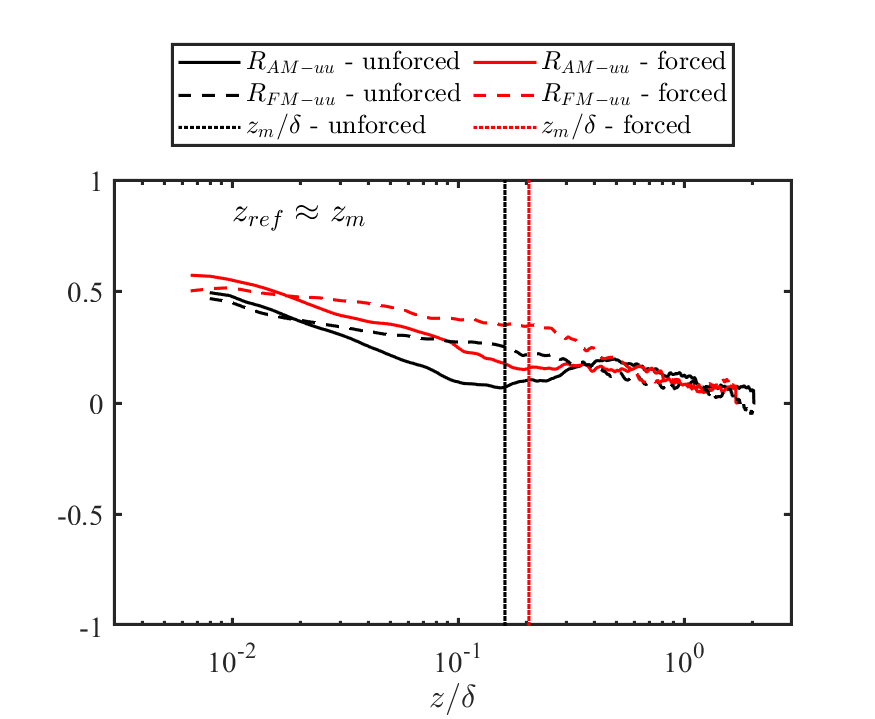
\includegraphics[width=0.55\textwidth]{pics/afosrAMFMuuzMax.png}
	\caption{Profiles of the amplitude $R_{AM-uu}$ and frequency $R_{FM-uu}$ modulation coefficient for the unforced (black lines) and forced (case B, red lines) flow derived from PIV based measurements. This shows the modulation effect of the large-scales at $z_{ref}\approx z_m$ (dotted lines) on the finer streamwise scales across the flow.}
	\label{fig:AMFMuuzMax}      
\end{figure}

\begin{figure}[h]
	\centering
	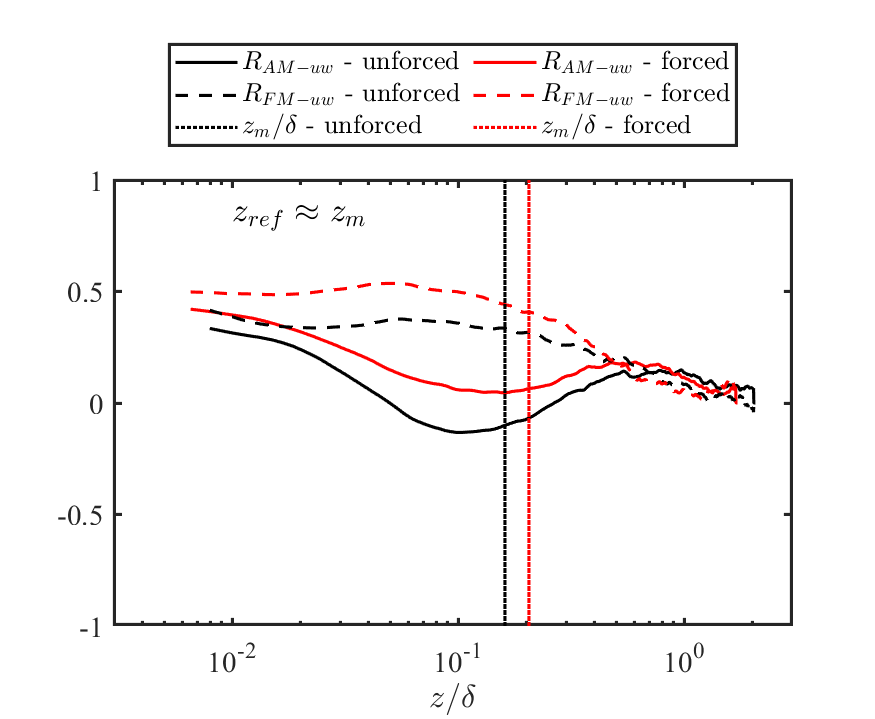
\includegraphics[width=0.55\textwidth]{pics/afosrAMFMuwzMax.png}
	\caption{Profiles of the amplitude $R_{AM-uw}$ and frequency $R_{FM-uw}$ modulation coefficient for the unforced (black lines) and forced (case B, red lines) flow derived from PIV based measurements. This shows the modulation effect of the large-scales at $z_{ref}\approx z_m$ (dotted lines) on the finer streamwise scales across the flow.}
	\label{fig:AMFMuwzMax}       
\end{figure}

However, the amplitude and frequency modulation coefficient $R_{AM}$ and $R_{FM}$ using the wavelet approach can quantify this interaction unambiguously. The streamwise large-scale at $z_{ref}\approx z_m$ is chosen as the reference large-scale $u_L$. The profiles of $R_{AM}$ and $R_{FM}$ with respect to this large-scale is shown in Figure~\ref{fig:AMFMuuzMax} and Figure\ref{fig:AMFMuwzMax}. Figure~\ref{fig:AMFMuuzMax} captures the modulation of the finer streamwise scales ($R_{AM-uu}$ and $R_{FM-uw}$) while Figure~\ref{fig:AMFMuwzMax} captures the modulation of the finer wall-normal scales ($R_{AM-uw}$ and $R_{FM-uw}$). These are shown for both the forced flow (case B) and the unforced flow. 

Considering the unforced flow, both $R_{AM-uu}$ and $R_{FM-uw}$ are highest in the very-near-wall region. This indicates that $u_L$ has a large modulating effect on the streamwise smaller scales in this region. The modulating effect gradually decreases as the distance from the wall increases. In the jet region, moving outwards from $z_m$, $R_{AM-uu}$ increases slightly and then decreases again. $R_{FM-uu}$ on the other hand gradually decreases from a maximum in the wall region moving outwards into the jet region. When forced the coupling between scales in the wall region is increased as indicated by an increase in $R_{AM-uu}$ as well as $R_{FM-uu}$ in this region. There is no perceptible change upon forcing in the outer jet region. 

The profiles of $R_{AM-uw}$ and $R_{FM-uw}$ are shown in Figure~\ref{fig:AMFMuwzMax}. $R_{AM-uw}$ like $R_{AM-uu}$ is a maximum in the wall region for the unforced flow, indicating significant coupling between the scales. Away from the wall, $R_{AM-uw}$ decreases and then becomes negative in the region around $z/\delta=0.1$. Moving outwards from the wall $R_{AM-uw}$ increases to become positive and then decreases slightly at the PWJ outer edge. When $z/\delta<0.1$, $R_{FM-uw}$ is maximum, positive and nearly a constant. $R_{FM-uw}$ while remaining positive gradually decreases into the jet region. When forced $R_{AM-uu}$ and $R_{FM-uu}$ both increase in the wall region with no perceptible change in the outer region. Together these observations emphasize that the large-scale, large-perturbation forcing considered altered the internal interactions of the flow, particularly the inner-outer interactions.